        %%******************************************%%
        %%                                          %%
        %%        Modello di tesi di laurea         %%
        %%            di Andrea Giraldin            %%
        %%                                          %%
        %%             2 novembre 2012              %%
        %%                                          %%
        %%******************************************%%


% I seguenti commenti speciali impostano:
% 1. 
% 2. PDFLaTeX come motore di composizione;
% 3. tesi.tex come documento principale;
% 4. il controllo ortografico italiano per l'editor.

% !TEX encoding = UTF-8
% !TEX TS-program = pdflatex
% !TEX root = tesi.tex
% !TEX spellcheck = it-IT

\documentclass[10pt,                    % corpo del font principale
               a4paper,                 % carta A4
               twoside,                 % impagina per fronte-retro
               openright,               % inizio capitoli a destra
               english,                 
               italian,                 
               ]{book}    

%**************************************************************
% Importazione package
%************************************************************** 

%\usepackage{amsmath,amssymb,amsthm}    % matematica

\usepackage{longtable}

\usepackage{multirow}

\usepackage{float}

\usepackage[T1]{fontenc}                % codifica dei font:
                                        % NOTA BENE! richiede una distribuzione *completa* di LaTeX

\usepackage[utf8]{inputenc}             % codifica di input; anche [latin1] va bene
                                        % NOTA BENE! va accordata con le preferenze dell'editor

\usepackage[english, italian]{babel}    % per scrivere in italiano e in inglese;
                                        % l'ultima lingua (l'italiano) risulta predefinita

\usepackage{bookmark}                   % segnalibri

\usepackage{caption}                    % didascalie

\usepackage{chngpage,calc}              % centra il frontespizio

\usepackage{csquotes}                   % gestisce automaticamente i caratteri (")

\usepackage{emptypage}                  % pagine vuote senza testatina e piede di pagina

\usepackage{epigraph}			% per epigrafi

\usepackage{eurosym}                    % simbolo dell'euro

%\usepackage{indentfirst}               % rientra il primo paragrafo di ogni sezione

\usepackage{graphicx}                   % immagini

\usepackage{newunicodechar}             % problemi con alcuni caratteri
\newunicodechar{fi}{fi}
\newunicodechar{ff}{ff}

\usepackage{hyperref}                   % collegamenti ipertestuali

\usepackage[binding=5mm]{layaureo}      % margini ottimizzati per l'A4; rilegatura di 5 mm

\usepackage{listings}                   % codici

\usepackage{microtype}                  % microtipografia

\usepackage{mparhack,fixltx2e,relsize}  % finezze tipografiche

\usepackage{nameref}                    % visualizza nome dei riferimenti                                      

\usepackage[font=small]{quoting}        % citazioni

\usepackage{subfig}                     % sottofigure, sottotabelle

\usepackage[italian]{varioref}          % riferimenti completi della pagina

\usepackage[dvipsnames]{xcolor}         % colori

\usepackage{booktabs}                   % tabelle                                       
\usepackage{tabularx}                   % tabelle di larghezza prefissata                                    
\usepackage{longtable}                  % tabelle su più pagine                                        
\usepackage{ltxtable}                   % tabelle su più pagine e adattabili in larghezza

\usepackage[toc, acronym]{glossaries}   % glossario
                                        % per includerlo nel documento bisogna:
                                        % 1. compilare una prima volta tesi.tex;
                                        % 2. eseguire: makeindex -s tesi.ist -t tesi.glg -o tesi.gls tesi.glo
                                        % 3. eseguire: makeindex -s tesi.ist -t tesi.alg -o tesi.acr tesi.acn
                                        % 4. compilare due volte tesi.tex.

\usepackage[backend=biber,style=verbose-ibid,hyperref,backref]{biblatex}
                                        % eccellente pacchetto per la bibliografia; 
                                        % produce uno stile di citazione autore-anno; 
                                        % lo stile "numeric-comp" produce riferimenti numerici
                                        % per includerlo nel documento bisogna:
                                        % 1. compilare una prima volta tesi.tex;
                                        % 2. eseguire: biber tesi
                                        % 3. compilare ancora tesi.tex.

%**************************************************************
% file contenente le impostazioni della tesi
%**************************************************************

%**************************************************************
% Frontespizio
%**************************************************************

% Comando per il nome dell'azienda

\newcommand{\visione}{VisioneImpresa}

% Contatore dei paragrafi

\setcounter{secnumdepth}{4}

% comando per i termini di Glossario

\newcommand{\glossaryItem}[1]{%
    \lowercase{\ifcsname @glsterms@\detokenize{#1}\endcsname}%
        #1%
    \else%
        \lowercase{\expandafter\gdef\csname @glsterms@\detokenize{#1}\endcsname{x}}%
        \emph{#1}\ped{G}%
    \fi%
}

% Comando per nuovo paragrafo

\newcommand{\myparagraph}[1]{\paragraph{#1}\mbox{} \mbox{}}


% Autore
\newcommand{\myName}{Tommaso Carraro}                                    
\newcommand{\myTitle}{Titolo della tesi}

% Tipo di tesi                   
\newcommand{\myDegree}{Tesi di laurea triennale}

% Università             
\newcommand{\myUni}{Università degli Studi di Padova}

% Facoltà       
\newcommand{\myFaculty}{Corso di Laurea in Informatica}

% Dipartimento
\newcommand{\myDepartment}{Dipartimento di Matematica "Tullio Levi-Civita"}

% Titolo del relatore
\newcommand{\profTitle}{Prof.}

% Relatore
\newcommand{\myProf}{Armir Bujari}

% Luogo
\newcommand{\myLocation}{Padova}

% Anno accademico
\newcommand{\myAA}{2017-2018}

% Data discussione
\newcommand{\myTime}{Dicembre 2018}


%**************************************************************
% Impostazioni di impaginazione
% see: http://wwwcdf.pd.infn.it/AppuntiLinux/a2547.htm
%**************************************************************

\setlength{\parindent}{14pt}   % larghezza rientro della prima riga
\setlength{\parskip}{0pt}   % distanza tra i paragrafi


%**************************************************************
% Impostazioni di biblatex
%**************************************************************
\bibliography{bibliografia} % database di biblatex 

\defbibheading{bibliography} {
    \cleardoublepage
    \phantomsection 
    \addcontentsline{toc}{chapter}{\bibname}
    \chapter*{\bibname\markboth{\bibname}{\bibname}}
}

\setlength\bibitemsep{1.5\itemsep} % spazio tra entry

\DeclareBibliographyCategory{opere}
\DeclareBibliographyCategory{web}

\addtocategory{opere}{womak:lean-thinking}
\addtocategory{web}{site:agile-manifesto}

\defbibheading{opere}{\section*{Riferimenti bibliografici}}
\defbibheading{web}{\section*{Siti Web consultati}}


%**************************************************************
% Impostazioni di caption
%**************************************************************
\captionsetup{
    tableposition=top,
    figureposition=bottom,
    font=small,
    format=hang,
    labelfont=bf
}

%**************************************************************
% Impostazioni di glossaries
%**************************************************************

%**************************************************************
% Acronimi
%**************************************************************
\renewcommand{\acronymname}{Acronimi e abbreviazioni}

\newacronym[description={\glslink{apig}{Application Program Interface}}]
    {api}{API}{Application Program Interface}

\newacronym[description={\glslink{umlg}{Unified Modeling Language}}]
    {uml}{UML}{Unified Modeling Language}

%**************************************************************
% Glossario
%**************************************************************
%\renewcommand{\glossaryname}{Glossario}

\newglossaryentry{apig}
{
    name=\glslink{api}{API},
    text=Application Program Interface,
    sort=api,
    description={in informatica con il termine \emph{Application Programming Interface API} (ing. interfaccia di programmazione di un'applicazione) si indica ogni insieme di procedure disponibili al programmatore, di solito raggruppate a formare un set di strumenti specifici per l'espletamento di un determinato compito all'interno di un certo programma. La finalità è ottenere un'astrazione, di solito tra l'hardware e il programmatore o tra software a basso e quello ad alto livello semplificando così il lavoro di programmazione}
}

\newglossaryentry{umlg}
{
    name=\glslink{uml}{UML},
    text=UML,
    sort=uml,
    description={in ingegneria del software \emph{UML, Unified Modeling Language} (ing. linguaggio di modellazione unificato) è un linguaggio di modellazione e specifica basato sul paradigma object-oriented. L'\emph{UML} svolge un'importantissima funzione di ``lingua franca'' nella comunità della progettazione e programmazione a oggetti. Gran parte della letteratura di settore usa tale linguaggio per descrivere soluzioni analitiche e progettuali in modo sintetico e comprensibile a un vasto pubblico}
}
 % database di termini
\makeglossaries


%**************************************************************
% Impostazioni di graphicx
%**************************************************************
\graphicspath{{immagini/}} % cartella dove sono riposte le immagini


%**************************************************************
% Impostazioni di hyperref
%**************************************************************
\hypersetup{
    %hyperfootnotes=false,
    %pdfpagelabels,
    %draft,	% = elimina tutti i link (utile per stampe in bianco e nero)
    colorlinks=true,
    linktocpage=true,
    pdfstartpage=1,
    pdfstartview=FitV,
    % decommenta la riga seguente per avere link in nero (per esempio per la stampa in bianco e nero)
    %colorlinks=false, linktocpage=false, pdfborder={0 0 0}, pdfstartpage=1, pdfstartview=FitV,
    breaklinks=true,
    pdfpagemode=UseNone,
    pageanchor=true,
    pdfpagemode=UseOutlines,
    plainpages=false,
    bookmarksnumbered,
    bookmarksopen=true,
    bookmarksopenlevel=1,
    hypertexnames=true,
    pdfhighlight=/O,
    %nesting=true,
    %frenchlinks,
    urlcolor=webbrown,
    linkcolor=RoyalBlue,
    citecolor=webgreen,
    %pagecolor=RoyalBlue,
    %urlcolor=Black, linkcolor=Black, citecolor=Black, %pagecolor=Black,
    pdftitle={\myTitle},
    pdfauthor={\textcopyright\ \myName, \myUni, \myFaculty},
    pdfsubject={},
    pdfkeywords={},
    pdfcreator={pdfLaTeX},
    pdfproducer={LaTeX}
}

%**************************************************************
% Impostazioni di itemize
%**************************************************************
\renewcommand{\labelitemi}{$\ast$}

%\renewcommand{\labelitemi}{$\bullet$}
%\renewcommand{\labelitemii}{$\cdot$}
%\renewcommand{\labelitemiii}{$\diamond$}
%\renewcommand{\labelitemiv}{$\ast$}


%**************************************************************
% Impostazioni di listings
%**************************************************************
\lstset{
    language=[LaTeX]Tex,%C++,
    keywordstyle=\color{RoyalBlue}, %\bfseries,
    basicstyle=\small\ttfamily,
    %identifierstyle=\color{NavyBlue},
    commentstyle=\color{Green}\ttfamily,
    stringstyle=\rmfamily,
    numbers=none, %left,%
    numberstyle=\scriptsize, %\tiny
    stepnumber=5,
    numbersep=8pt,
    showstringspaces=false,
    breaklines=true,
    frameround=ftff,
    frame=single
} 


%**************************************************************
% Impostazioni di xcolor
%**************************************************************
\definecolor{webgreen}{rgb}{0,.5,0}
\definecolor{webbrown}{rgb}{.6,0,0}


%**************************************************************
% Altro
%**************************************************************

\newcommand{\omissis}{[\dots\negthinspace]} % produce [...]

% eccezioni all'algoritmo di sillabazione
\hyphenation
{
    ma-cro-istru-zio-ne
    gi-ral-din
}

\newcommand{\sectionname}{sezione}
\addto\captionsitalian{\renewcommand{\figurename}{Figura}
                       \renewcommand{\tablename}{Tabella}}

\newcommand{\glsfirstoccur}{\ap{{[g]}}}

\newcommand{\intro}[1]{\emph{\textsf{#1}}}

%**************************************************************
% Environment per ``rischi''
%**************************************************************
\newcounter{riskcounter}                % define a counter
\setcounter{riskcounter}{0}             % set the counter to some initial value

%%%% Parameters
% #1: Title
\newenvironment{risk}[1]{
    \refstepcounter{riskcounter}        % increment counter
    \par \noindent                      % start new paragraph
    \textbf{\arabic{riskcounter}. #1}   % display the title before the 
                                        % content of the environment is displayed 
}{
    \par\medskip
}

\newcommand{\riskname}{Rischio}

\newcommand{\riskdescription}[1]{\textbf{\\Descrizione:} #1.}

\newcommand{\risksolution}[1]{\textbf{\\Soluzione:} #1.}

%**************************************************************
% Environment per ``use case''
%**************************************************************
\newcounter{usecasecounter}             % define a counter
\setcounter{usecasecounter}{0}          % set the counter to some initial value

%%%% Parameters
% #1: ID
% #2: Nome
\newenvironment{usecase}[2]{
    \renewcommand{\theusecasecounter}{\usecasename #1}  % this is where the display of 
                                                        % the counter is overwritten/modified
    \refstepcounter{usecasecounter}             % increment counter
    \vspace{10pt}
    \par \noindent                              % start new paragraph
    {\large \textbf{\usecasename #1: #2}}       % display the title before the 
                                                % content of the environment is displayed 
    \medskip
}{
    \medskip
}

\newcommand{\usecasename}{UC}

\newcommand{\usecaseactors}[1]{\textbf{\\Attori Principali:} #1. \vspace{4pt}}
\newcommand{\usecasepre}[1]{\textbf{\\Precondizioni:} #1. \vspace{4pt}}
\newcommand{\usecasedesc}[1]{\textbf{\\Descrizione:} #1. \vspace{4pt}}
\newcommand{\usecasepost}[1]{\textbf{\\Postcondizioni:} #1. \vspace{4pt}}
\newcommand{\usecasealt}[1]{\textbf{\\Scenario Alternativo:} #1. \vspace{4pt}}

%**************************************************************
% Environment per ``namespace description''
%**************************************************************

\newenvironment{namespacedesc}{
    \vspace{10pt}
    \par \noindent                              % start new paragraph
    \begin{description} 
}{
    \end{description}
    \medskip
}

\newcommand{\classdesc}[2]{\item[\textbf{#1:}] #2}                     % file con le impostazioni personali

\begin{document}
%**************************************************************
% Materiale iniziale
%**************************************************************
\frontmatter
% !TEX encoding = UTF-8
% !TEX TS-program = pdflatex
% !TEX root = ../tesi.tex

%**************************************************************
% Frontespizio 
%**************************************************************
\begin{titlepage}

\begin{center}

\begin{LARGE}
\textbf{\myUni}\\
\end{LARGE}

\vspace{10pt}

\begin{Large}
\textsc{\myDepartment}\\
\end{Large}

\vspace{10pt}

\begin{large}
\textsc{\myFaculty}\\
\end{large}

\vspace{30pt}
\begin{figure}[htbp]
\begin{center}

\includegraphics[height=6cm]{logo-unipd}
\end{center}
\end{figure}
\vspace{30pt} 

\begin{LARGE}
\begin{center}
\textbf{\myTitle}\\
\end{center}
\end{LARGE}

\vspace{10pt} 

\begin{large}
\textsl{\myDegree}\\
\end{large}

\vspace{40pt} 

\begin{large}
\begin{flushleft}
\textit{Relatore}\\ 
\vspace{5pt} 
\profTitle \myProf
\end{flushleft}

\vspace{0pt} 

\begin{flushright}
\textit{Laureando}\\ 
\vspace{5pt} 
\myName
\end{flushright}
\end{large}

\vspace{40pt}

\line(1, 0){338} \\
\begin{normalsize}
\textsc{Anno Accademico \myAA}
\end{normalsize}

\end{center}
\end{titlepage} 
% !TEX encoding = UTF-8
% !TEX TS-program = pdflatex
% !TEX root = ../tesi.tex

%**************************************************************
% Colophon
%**************************************************************
\clearpage
\phantomsection
\thispagestyle{empty}

\hfill

\vfill

\noindent\myName: \textit{\myTitle,}
\myDegree,
\textcopyright\ \myTime.
% !TEX encoding = UTF-8
% !TEX TS-program = pdflatex
% !TEX root = ../tesi.tex

%**************************************************************
% Dedica
%**************************************************************
\cleardoublepage
\phantomsection
\thispagestyle{empty}
\pdfbookmark{Dedica}{Dedica}

\vspace*{3cm}

\begin{center}
Lorem ipsum dolor sit amet, consectetuer adipiscing elit. \\ \medskip
--- Oscar Wilde    
\end{center}

\medskip

\begin{center}
Dedicato a ...
\end{center}

% !TEX encoding = UTF-8
% !TEX TS-program = pdflatex
% !TEX root = ../tesi.tex

%**************************************************************
% Sommario
%**************************************************************
\cleardoublepage
\phantomsection
\pdfbookmark{Sommario}{Sommario}
\begingroup
\let\clearpage\relax
\let\cleardoublepage\relax
\let\cleardoublepage\relax

\chapter*{Sommario}

Il presente documento descrive il lavoro svolto durante il periodo di \textit{stage}, della durata di 320 ore, dal laureando Tommaso Carraro presso l'azienda \visione{} S.r.l. situata a Pernumia (PD).

Lo scopo principale del progetto era la realizzazione di un'applicazione \textit{mobile} che permettesse ai clienti di una qualsiasi azienda di acquistare, tramite il proprio \textit{smartphone}, dei prodotti venduti dalla stessa. Per raggiungere questo fine sono stati assegnati vari compiti.

Lo studente ha dovuto scegliere in autonomia l'ambiente di sviluppo ritenuto più opportuno. Poiché era richiesto che l'applicazione funzionasse sia in ambiente \textit{Android} che in ambiente \textit{iOS}, si è dovuto scegliere un \glossaryItem{framework cross-platfrom} e, in particolare, il \glossaryItem{framework} \textit{PhoneGap}.

In seguito alla scelta del \textit{framework} vi è stato un periodo di formazione, di circa 40 ore, sui \textit{software} gestionali utilizzati in azienda e sul linguaggio \textit{JavaScript}, in modo da facilitare lo sviluppo del progetto.

Si è poi potuto proseguire con la progettazione delle varie componenti della \glossaryItem{piattaforma}, quali \glossaryItem{servizio web}, \textit{database} sottostanti, logica applicativa e interfaccia grafica. 
L'applicazione doveva funzionare interamente \textit{online}, nessun dato doveva essere memorizzato in locale, per cui il servizio \textit{web} e i \textit{database} sono stati installati su un \textit{server} \glossaryItem{Azure} di proprietà dell'azienda.
In particolare, è stato richiesto di progettare un \textit{database} che permettesse la gestione dei dati di autenticazione e un \textit{database} che contenesse i dati utili alla gestione degli ordini presso un'azienda cliente. Il \textit{database} contenente i dati proprietari dell'azienda poteva essere locale al \textit{server Azure} o all'interno di un \textit{server cloud} dell'azienda stessa, a seconda delle scelte effettuate da quest'ultima.

In seguito alla progettazione delle varie parti si è iniziata l'implementazione della piattaforma. Il servizio doveva gestire le richieste \glossaryItem{HTTP} (\textit{HyperText Transfer Protocol}) provenienti dall'applicazione tramite oggetti \glossaryItem{servlet} \textit{Java} e rispondere a queste mediante stringhe in formato \glossaryItem{JSON}.
La logica applicativa dell'applicazione doveva essere scritta in linguaggio \textit{JavaScript}, questo perché lo stagista ha scelto il \textit{framework PhoneGap}. Per permettere all'applicazione di comunicare con il servizio \textit{web} tramite richieste \textit{HTTP}, si è dovuta utilizzare la tecnica \glossaryItem{AJAX} (\textit{Asynchronous JavaScript And XML}).
Il \textit{design} dell'interfaccia doveva essere simile al \textit{design} di un'altra applicazione sviluppata dall'azienda, chiamata \glossaryItem{moviDOC}. Infine, per permettere all'applicazione di essere \glossaryItem{usabile} dalla maggior parte dei dispositivi, si è dovuto rendere il \textit{design} della stessa \glossaryItem{responsive}.

%\vfill
%
%\selectlanguage{english}
%\pdfbookmark{Abstract}{Abstract}
%\chapter*{Abstract}
%
%\selectlanguage{italian}

\endgroup			

\vfill


% !TEX encoding = UTF-8
% !TEX TS-program = pdflatex
% !TEX root = ../tesi.tex

%**************************************************************
% Ringraziamenti
%**************************************************************
\cleardoublepage
\phantomsection
\pdfbookmark{Ringraziamenti}{ringraziamenti}

\begin{flushright}{
	\slshape    
	``Life is really simple, but we insist on making it complicated''} \\ 
	\medskip
    --- Confucius
\end{flushright}


\bigskip

\begingroup
\let\clearpage\relax
\let\cleardoublepage\relax
\let\cleardoublepage\relax

\chapter*{Ringraziamenti}

\noindent \textit{Innanzitutto, vorrei esprimere la mia gratitudine al Dott. Armir Bujari, relatore della mia tesi, per l'aiuto e il sostegno fornitomi durante la stesura del lavoro e per avermi ricevuto nel suo ufficio ogniqualvolta gli è stato possibile.}\\

\noindent \textit{Ringrazio il mio tutor aziendale, Francesco Turra, per avermi dato la possibilità di lavorare a \visione{}, ma soprattutto per avermi assegnato un progetto a cui ero interessato. Non lo ringrazierò mai abbastanza per avermi concesso di lavorare da casa alcuni giorni mentre preparavo un esame importante, e per avermi aiutato ad ottenere la borsa di studio ``Mille e una lode'', prolungando di un mese il periodo di stage.}\\

\noindent \textit{Merita di essere nominato il mio collega Luca, sviluppatore di \visione{}, senza l'aiuto del quale non avrei terminato il progetto nei tempi prestabiliti. La sua esperienza mi ha permesso di risolvere gran parte dei problemi riscontrati durante lo sviluppo del progetto.}\\

\noindent \textit{Desidero ringraziare con affetto mia madre Federica, mio padre Gianni e mio fratello Edoardo, per il sostegno e il grande aiuto ricevuti durante questi anni di studio, ma soprattutto per la grande pazienza dimostrata nei periodi più impegnativi di questo terzo anno, durante il quale non sono sempre stato presente.}\\

\noindent \textit{Ringrazio infinitamente il Professor Tullio Vardanega per avermi aiutato ad ottenere la borsa di studio ``Mille e una lode'' e per aver risposto tempestivamente a tutte le mail concernenti l'argomento.}\\

\noindent \textit{Ringrazio il mio collega universitario Alberto per avermi aiutato a preparare tutti gli esami durante questi anni di studio a Padova.}\\

\noindent \textit{Ringrazio i miei cari amici Margherita e Gabriele per essermi sempre stati accanto e per il conforto ricevuto durante i momenti cupi della mia vita.}\\

\noindent \textit{Ho desiderio di ringraziare poi la ``BMX family'', che alimenta ogni giorno la passione che covo per questo bellissimo sport e stile di vita.}\\

\noindent \textit{Ringrazio infine Elisa, la ragazza che ho amato e con la quale ho passato i momenti più belli di questo 2018.}
\bigskip

\noindent\textit{\myLocation{}, 10 \myTime{}}
\hfill \myName

\endgroup


% !TEX encoding = UTF-8
% !TEX TS-program = pdflatex
% !TEX root = ../tesi.tex

%**************************************************************
% Indici
%**************************************************************
\cleardoublepage
\pdfbookmark{\contentsname}{tableofcontents}
\setcounter{tocdepth}{2}
\tableofcontents
%\markboth{\contentsname}{\contentsname} 
\clearpage

\begingroup 
    \let\clearpage\relax
    \let\cleardoublepage\relax
    \let\cleardoublepage\relax
    %*******************************************************
    % Elenco delle figure
    %*******************************************************    
    \phantomsection
    \pdfbookmark{\listfigurename}{lof}
    \listoffigures

    \vspace*{8ex}

    %*******************************************************
    % Elenco delle tabelle
    %*******************************************************
    \phantomsection
    \pdfbookmark{\listtablename}{lot}
    \listoftables
        
    \vspace*{8ex}
\endgroup

\cleardoublepage

\cleardoublepage

%**************************************************************
% Materiale principale
%**************************************************************
\mainmatter
% !TEX encoding = UTF-8
% !TEX TS-program = pdflatex
% !TEX root = ../tesi.tex

%**************************************************************
\chapter{Introduzione}
\label{cap:introduzione}
%**************************************************************

Al giorno d'oggi la tecnologia sta ricoprendo un ruolo importante nei \textit{task} di tutti i giorni. In particolare, è indispensabile che un'azienda venditrice di un qualsiasi tipo di prodotti abbia una propria \glossaryItem{piattaforma} \textit{online} per la gestione degli ordini. Questo perché le persone sono sempre più abituate ad effettuare ordini \textit{online}. Infatti, acquistare \textit{online} risulta vantaggioso per molteplici motivi, quali il risparmio di tempo e denaro ma soprattutto la comodità di non doversi muovere da casa per acquistare un prodotto. Per molte aziende non cogliere questo cambiamento potrebbe essere fallimentare, infatti, in futuro, la maggior parte degli acquisti avverrà principalmente \textit{online} per qualsiasi tipologia di prodotto. 

\textit{MoviORDER} nasce per rispondere a questa necessità, proponendosi come piattaforma universale per la registrazione e l'invio di ordini \textit{online}. Una qualsiasi azienda interessata a vendere i propri prodotti \textit{online} può contattare \visione{} per ricevere \textit{moviORDER} e, dopo un breve periodo di configurazione, l'applicazione sarà pronta a ricevere ordini dagli utenti registrati. 
\textit{MoviORDER} risulta vantaggiosa per i seguenti motivi:
\begin{itemize}
	\item per i clienti:
	\begin{itemize}
		\item possibilità di trovare i prodotti \textit{online} e non solamente nel negozio fisico;
		\item possibilità di risparmiare tempo e denaro dovuti al raggiungimento del negozio fisico;
		\item possibilità di controllare in tempo reale la disponibilità dei prodotti.
	\end{itemize}
	\item per le aziende:
	\begin{itemize}
		\item riduce il rischio di fallimento dovuto al cambiamento delle convenzioni degli utenti;
		\item aumenta il numero di clienti per l'azienda, permettendo a coloro che non riescono a raggiungere il negozio fisico di poter comunque effettuare ordini grazie alla piattaforma \textit{online}.
	\end{itemize}
\end{itemize}

%**************************************************************
\section{L'azienda}

\visione{} è un'azienda che da 30 anni si occupa di informatica e più precisamente di quella parte dell'informatica dedicata alle applicazioni gestionali. Inizialmente l'attività di \visione{} era rivolta ad aziende, enti pubblici, studi professionali e centri di elaborazione dati, gestendo totalmente problematiche informatiche, progettazione di sistemi, \textit{hardware}, reti, sistemi operativi e \textit{software} applicativo. Oggi \visione{} punta sulla specializzazione, dedicandosi in modo particolare allo sviluppo del \textit{software} applicativo e dei relativi servizi di implementazione dello stesso nell'azienda. \visione{} è un team di persone esperte e motivate che opera direttamente su gran parte del Nord Est e indirettamente sull'intero territorio nazionale. \visione{} si rivolge a piccole e medie aziende italiane che intendono impostare sul sistema informatico non solo la semplice gestione amministrativa o di magazzino, ma la completa organizzazione aziendale per affrontare un futuro sempre più complesso e veloce, con il supporto di un sistema informatico che aiuti l'azienda a prendere decisioni sempre basate su dati precisi.

\begin{figure}[!h] 
    \centering 
    
\includegraphics[width=0.6\columnwidth]{visione/logoVisione} 
    \caption{Logo dell'azienda \visione{}}
\end{figure}

\subsection{Core business}

\visione{} presenta principalmente due core business: \textit{VisionENTERPRISE} e \textit{movidat}. \textit{VisionENTERPRISE} è un \glossaryItem{software gestionale} \glossaryItem{ERP} dedicato alle medie e piccole aziende industriali, commerciali e dei servizi, che gestiscono notevoli moli di dati e hanno la necessità di lavorare con grande velocità e stabilità. Il \textit{software} è in grado di collegarsi a tutte le informazioni dell'azienda cliente e di interfacciarsi con tutti i \textit{software} utilizzati al fine di gestire in modo ottimale l'intera organizzazione aziendale con la massima semplicità e velocità operativa. Il \textit{software} è in grado di rendere disponibile in tempo reale, alla direzione o al titolare dell'azienda, tutte le informazioni di cui hanno bisogno per prendere decisioni sulla base di dati concreti e oggettivi. Altra qualità di \textit{VisionENTERPRISE} è la sua completa copertura funzionale: dalla contabilità al magazzino, dall'area commerciale alla produzione, dal controllo di gestione all'\textit{E-business}.

\begin{figure}[!h] 
    \centering 
    
\includegraphics[width=0.8\columnwidth]{visione/visionEnterprise} 
    \caption{Banner del \textit{software} \textit{VisionENTERPRISE}}
\end{figure}

\textit{Movidat} è un marchio di \visione{} che progetta e sviluppa applicazioni per dispositivi mobile rivolte alle piccole e medie imprese che vogliono rendere i loro \glossaryItem{processi} più semplici, veloci ed efficienti. Lo slogan di \textit{movidat} è ``ovunque tu sia, il tuo business a portata di mano!'', infatti le applicazioni \textit{movidat} sono rivolte ai dipendenti che lavorano in movimento, i quali devono essere in grado di agire tempestivamente in caso di problematiche inaspettate. Le soluzioni \textit{movidat} sono compatibili con la maggior parte dei \textit{software} gestionali disponibili sul mercato. Tra le soluzioni di miglior successo vi sono:
\begin{itemize}
	\item \textbf{\textit{moviCheck}}: applicazione rivolta alle aziende che vogliono offrire alle proprie figure direzionali uno strumento in grado di analizzare in mobilità i dati di business più significativi;
	\item \textbf{\textit{moviSell}}: applicazione specificatamente rivolta ai professionisti della vendita, ideata come supporto per la gestione dei rapporti con i clienti.
\end{itemize}

\begin{figure}[!h] 
    \centering 
    
\includegraphics[width=0.6\columnwidth]{visione/movidat} 
    \caption{Logo del marchio \textit{movidat}}
\end{figure}

\textit{MoviORDER} rientra tra le applicazioni del marchio \textit{movidat}, soddisfacendo però i bisogni del cliente finale dell'azienda. Infatti, tramite moviORDER, gli utenti possono acquistare dei prodotti della propria azienda direttamente \textit{online}, senza doversi recare al negozio fisico.

%**************************************************************
\section{Offerta di stage}

Il 10 Aprile 2018 si è tenuta a Padova la 15-esima edizione di \textit{Stage-IT}, iniziativa che mira ad agevolare l'incontro tra aziende e studenti universitari che puntano ad entrare nel mondo del lavoro con specifico riferimento al settore \glossaryItem{ICT}, favorendo un'occasione di conoscenza reciproca tramite colloqui individuali. Le aziende partecipanti propongono spesso progetti innovativi con ottime opportunità di accrescimento delle competenze individuali. Proprio per questo motivo, lo stagista ha deciso di partecipare attivamente all'evento, concludendo positivamente sette colloqui. 

\begin{figure}[!h] 
    \centering 
    
\includegraphics[width=0.8\columnwidth]{loghi/stage} 
    \caption{Logo dell'evento \textit{Stage-IT}}
\end{figure}

Le aziende sono state selezionate dallo studente per ambito e tecnologie di sviluppo adottate nel progetto. In particolare, lo studente era in cerca di:
\begin{itemize}
	\item progetti di sviluppo in ambito mobile (preferibilmente \textit{Android}): al giorno d'oggi i task si stanno spostando sempre di più dalle postazioni desktop ai dispositivi portatili;
	\item progetti di sviluppo di \glossaryItem{applicazioni web} (preferibilmente con utilizzo di \textit{framework} e \glossaryItem{librerie} \textit{Javascript} moderne): le \textit{skill} di programmazione in \textit{Javascript} sono richieste da gran parte delle aziende che si occupano della realizzazione di applicazioni \textit{web}.
\end{itemize}
Tra le varie offerte di \textit{stage}, \visione{} rientrava in entrambe le preferenze, infatti proponeva un progetto di sviluppo in ambito mobile con l'utilizzo di un \textit{framework cross-platform}. Nonostante lo \textit{stage} non prevedesse lo sviluppo in \glossaryItem{codice nativo} \textit{Android}, permetteva comunque la realizzazione di un'applicazione mobile. Inoltre, richiedendo il progetto l'utilizzo di un \textit{framework cross-platform}, era pressoché implicito l'utilizzo di \glossaryItem{tecnologie web}, tra le quali anche \textit{Javascript}. Per cui, il buon compromesso tra tecnologie conosciute e tecnologie ritenute interessanti ha favorito \visione{} tra le varie offerte analizzate.

\newpage

\section{Obiettivi e pianificazione}

Il progetto prevedeva la realizzazione di un'applicazione mobile, principalmente \textit{Android} e \textit{iOS}, che consentisse ad un utente registrato, tramite la lettura di codici a barre o l'inserimento manuale di codici articolo, di inviare ordini di acquisto al proprio fornitore. L'azienda ha richiesto lo sviluppo delle seguenti funzionalità:
\begin{itemize}
	\item \textbf{\textit{login}}: permette ad un utente di essere riconosciuto come cliente dell'azienda. Le credenziali di accesso vengono distribuite dall'azienda insieme all'applicazione;
	\item \textbf{gestione del carrello}:
	\begin{itemize}
		\item \textbf{aggiunta di un nuovo articolo}: permette all'utente autenticato di aggiungere un nuovo articolo al carrello. L'aggiunta di un nuovo articolo prevede l'inserimento di un codice articolo, tramite scansione di un codice a barre o inserimento manuale e, successivamente, l'inserimento di una quantità da ordinare;
		\item \textbf{modifica di un articolo}: permette all'utente autenticato di modificare la quantità di un articolo in carrello;
		\item \textbf{selezione articoli}: permette all'utente autenticato di selezionare uno o più articoli in carrello;
		\item \textbf{deselezione articoli}: permette all'utente autenticato di deselezionare uno o più articoli in carrello;
		\item \textbf{rimozione articoli}: permette all'utente autenticato di rimuovere gli articoli selezionati dal carrello;
		\item \textbf{invio ordine}: permette all'utente autenticato di inviare un ordine composto dagli articoli selezionati in carrello.
	\end{itemize}
	\item \textbf{invio di e-mail di conferma}: nel caso in cui un ordine venga inviato con successo, il sistema deve inviare all'azienda e all'utente autenticato una mail di conferma contenente un riepilogo dell'ordine.
\end{itemize}

I prodotti attesi per il termine dello \textit{stage} erano:
\begin{itemize}
	\item \textbf{analisi dei requisiti} per l'applicazione da realizzare: partendo dalle specifiche e dalla microanalisi ricevuta, lo stagista doveva definire le funzionalità offerte dall'applicazione, i dettagli dei \textit{web services} di comunicazione tra \textit{database} e \textit{front end}, e l'interfaccia grafica dell'applicazione;
	\item \textbf{applicazione \textit{moviORDER}}: sviluppo dell'applicazione in ambiente \glossaryItem{multipiattaforma} in seguito alla scelta del \textit{framework} ritenuto più opportuno;
	\item \textbf{servizio \textit{web}}: sviluppo di un servizio \textit{web} che permettesse all'applicazione di accedere ed interagire con un \textit{database} su un \textit{server cloud} di \visione{};
	\item \textbf{manuali} utente e sviluppatore. 
\end{itemize}

Per adempiere a questi obblighi lo stagista ha pianificato delle attività che sono state concordate con il tutor aziendale. Lo \textit{stage} prevedeva 320 ore di lavoro che sono state distribuite nel periodo tra l'inizio e la fine dello \textit{stage}, 2 Luglio 2018 e 7 Settembre 2018 rispettivamente. La pianificazione oraria delle attività all'inizio dello \textit{stage} è indicata nella seguente tabella.

{\renewcommand{\arraystretch}{2}
\begin{center}
\begin{longtable}{ | >{\arraybackslash}p{11cm} | >{\centering\arraybackslash}p{1cm} | }
        
\hline
\textbf{Attività} & \textbf{Ore} \\ \hline
\endhead
Formazione assistita sui \textit{software} gestionali di \visione{} e sulle applicazioni analoghe a \textit{moviORDER} & 40 \\ \hline
Formazione individuale sui \textit{framework cross-platform} e scelta del \textit{framework} ritenuto più opportuno & 40 \\ \hline
Ridefinizione delle specifiche comprendente delle soluzioni da realizzare e delle metodologie per implementarle & 40 \\ \hline
Realizzazione dei \textit{web services} per l'interazione con il \textit{database}: servizio di autenticazione, servizio di lettura dati, servizio di scrittura dati e servizio di invio e-mail & 40 \\ \hline
Realizzazione della \textit{business logic} dell'applicazione & 40 \\ \hline
Realizzazione delle interfacce grafiche dell'applicazione: \textit{login}, gestione carrello, aggiunta/modifica articolo e invio ordine & 40 \\ \hline
Test di scambio dati tra \textit{VisionENTERPRISE} e \textit{moviORDER} & 40 \\ \hline
Documentazione del codice e stesura del manuale utente e sviluppatore & 40 \\
\hline
\caption{Pianificazione oraria del periodo di \textit{stage}}
\end{longtable}
\end{center}}

Viene di seguito riportato un \glossaryItem{diagramma di Gantt} che illustra come le attività di \textit{stage} sono state allocate nel tempo di calendario da parte dello stagista. Il diagramma mostra le dipendenze temporali tra le varie attività e il periodo di ferie che l'azienda ha concesso allo stagista, indicato in viola.

\begin{figure}[!h] 
    \centering 
    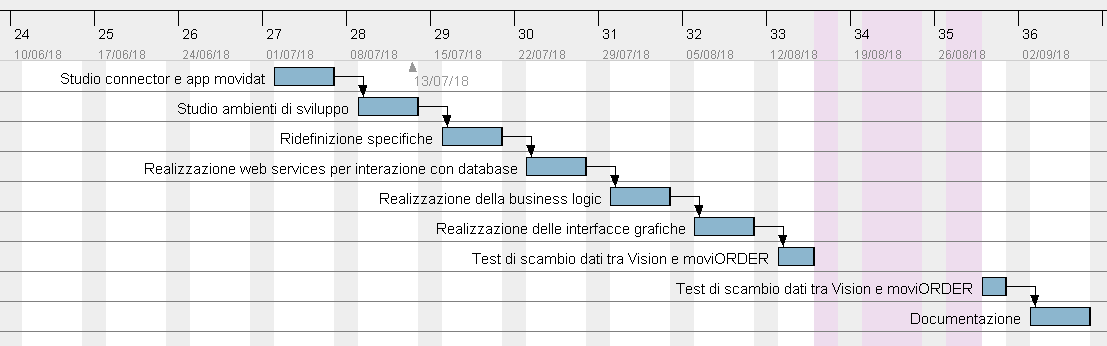
\includegraphics[width=\columnwidth]{diagrammi/pianificazione} 
    \caption{Diagramma di \textit{Gantt} della pianificazione delle attività di \textit{stage}}
\end{figure}

\newpage

\section{Rischi}

Parallelamente allo studio dei documenti forniti dal tutor aziendale, è stata sviluppata un'analisi preventiva dei rischi che si sarebbero potuti verificare durante lo svolgimento delle attività di progetto. Al fine di attuare una corretta e quindi utile gestione dei rischi, essi sono stati identificati nel contesto di processo e di prodotto. In seguito all'identificazione dei rischi sono state analizzate le probabilità di occorrenza, imminenza e l'impatto di ciascun rischio, pianificando come evitarne o mitigarne gli effetti. Durante lo svolgimento del progetto è stato costantemente eseguito un controllo per rilevare eventuali indicatori di rischio e ogni nuovo rischio rilevato è stato aggiunto alla seguente tabella, insieme alle azioni atte a mitigarne gli effetti.

\begin{small}
    \begin{center}
        \renewcommand{\arraystretch}{2}
        \begin{longtable}{| >{\centering\arraybackslash}p{1.5cm} | >{\arraybackslash}p{4cm} | >{\centering\arraybackslash} p{2cm} | >{\arraybackslash} p{3.75cm}|}
        	\hline
            \textbf{Rischio} & \textbf{Descrizione} & \textbf{Grado} & \textbf{Mitigazione} \\
            \hline
            \endhead
            
            Tecnologie non conosciute
            &
            Il tempo richiesto per l'apprendimento delle nuove tecnologie da parte dello stagista
            potrebbe causare ritardi nello sviluppo
            &
            Occorrenza: \textbf{Media} Pericolosità: \textbf{Media}
            &
            Effettuare una buona analisi iniziale delle tecnologie richieste ed usufruire del tempo di formazione per prendere dimestichezza con le tecnologie non conosciute
         	\\
            \hline
            
            Modifica dei requisiti
            &
            Nonostante i requisiti esposti inizialmente siano chiari, vi è la possibilità
            che questi vengano modificati dal tutor aziendale
            &
            Occorrenza: \textbf{Bassa} Pericolosità: \textbf{Alta}
            & 
            Negoziare la modifica ai requisiti nel caso in cui siano richiesti cambiamenti eccessivi da parte del tutor aziendale
            \\
            \hline
            
            Stima dei tempi
            &
            Può accadere che lo stagista abbia pianificato erroneamente alcune attività e che durante lo sviluppo si sforino i tempi concordati
            &
            Occorrenza: \textbf{Media} Pericolosità: \textbf{Alta}
            & 
            Agire tempestivamente sulla pianificazione, ove possibile, nei casi più gravi. Pianificare in maniera intelligente inserendo dei \glossaryItem{periodi di slack} tra le attività ritenute più critiche
            \\
            \hline
            
            Difficoltà nelle interazioni
            &
            Durante lo \textit{stage} le interazioni avvengono spesso tramite scambio di e-mail tra lo stagista e il tutor aziendale. Può succedere che alcune risposte arrivino in tempi prolungati, causando tempi morti nello sviluppo dell'applicazione
            &
            Occorrenza: \textbf{Bassa} Pericolosità: \textbf{Media}
            & 
            Se il problema dovesse diventare ingestibile, proporre al tutor aziendale l'utilizzo di uno strumento di comunicazione alternativo, altrimenti presentarsi fisicamente in ufficio per discutere delle problematiche di maggiore entità
            \\
            \hline
            \caption{Analisi dei rischi}
        \end{longtable}
    \end{center}
\end{small}


%**************************************************************
\section{Organizzazione del testo}

\begin{description}
    \item[{\hyperref[cap:processi-metodologie]{Il secondo capitolo}}] descrive il modello di \glossaryItem{ciclo di vita} adottato durante lo sviluppo del progetto.
    
    \item[{\hyperref[background]{Il terzo capitolo}}] descrive le tecnologie utilizzate durante lo sviluppo del progetto.
    
    \item[{\hyperref[cap:analisi-requisiti]{Il quarto capitolo}}] descrive i \glossaryItem{casi d'uso} e i corrispondenti requisiti rilevati durante la fase di analisi dei requisiti del progetto.
    
    \item[{\hyperref[cap:progettazione-codifica]{Il quinto capitolo}}] descrive l'\glossaryItem{architettura} dell'applicazione, comprensiva di contestualizzazione dei \glossaryItem{design pattern} adottati.
    
    \item[{\hyperref[codifica]{Il sesto capitolo}}] descrive i dettagli implementativi del progetto.
    
    \item[{\hyperref[cap:verifica-validazione]{Il settimo capitolo}}] descrive i processi di verifica e validazione attuati nel progetto.
    
    \item[{\hyperref[cap:conclusioni]{L'ottavo capitolo}}] descrive le conclusioni tratte dallo studente in merito al progetto realizzato.
\end{description}

Riguardo la stesura del testo, relativamente al documento, sono state adottate le seguenti convenzioni tipografiche:
\begin{itemize}
	\item gli acronimi, le abbreviazioni e i termini ambigui o di uso non comune menzionati vengono definiti nel glossario, situato alla fine del presente documento;
	\item per la prima occorrenza dei termini riportati nel glossario viene utilizzata la seguente nomenclatura: \glossaryItem{termine};
	\item i termini in lingua straniera, o facenti parti del gergo tecnico, sono evidenziati con il carattere \emph{corsivo}.
\end{itemize}             % Introduzione
% !TEX encoding = UTF-8
% !TEX TS-program = pdflatex
% !TEX root = ../tesi.tex

%**************************************************************
\chapter{Processo di sviluppo}
\label{cap:processi-metodologie}
%**************************************************************

Durante lo sviluppo di un progetto software è importante aderire ad un modello di \glossaryItem{ciclo di vita}. La durata del ciclo di vita di un software inizia dalla sua concezione, ossia il momento in cui nasce il bisogno, passa poi per lo sviluppo e l'utilizzo, prolungato nel tempo e in cui è soggetto a manutenzione, per poi terminare con il ritiro del prodotto. L'avanzamento tra questi stati avviene tramite l'esecuzione di attività definite nel modello di ciclo di vita adottato. I progetti in cui non viene adottato un modello di ciclo di vita sono detti \glossaryItem{code-n-fix} e l'insieme delle attività è priva di organizzazione e rende il progetto caotico e poco gestibile. Aderire ad un modello di ciclo di vita è quindi essenziale ma determina vincoli sulla pianificazione e sulla gestione di progetto, per cui è importante che la scelta del modello da adottare avvenga prima della pianificazione del progetto. In un modello di ciclo di vita le attività sono coese e raggruppate in processi e gli ingressi e le uscite di ciascuna attività sono identificati, al fine di permettere un ordinamento temporale tra esse.

%**************************************************************
\section{Modello incrementale}

Durante il corso di Ingegneria del Software sono stati studiati vari modelli di ciclo di vita. In particolare, viste le modalità di interazione e le richieste del tutor aziendale, per il progetto di stage poteva essere adottato un modello incrementale o una metodologia \glossaryItem{Agile}. Non avendo l'azienda imposto un processo di sviluppo, lo stagista ha optato per il modello incrementale in quanto già utilizzato durante il progetto di Ingegneria del Software. Tale modello segue un approccio adattativo dove la realtà è considerata imprevedibile e per questo risulta utile nel caso in cui i requisiti possano cambiare in corso d'opera. Il modello presenta una fase iniziale di analisi e progettazione dove il problema viene compreso nel suo contorno fondamentale individuando i requisiti macroscopici e l'architettura del prodotto. Tale fase non viene ripetuta e risulta essenziale per la pianificazione dei cicli di \glossaryItem{incremento} in cui si decide il numero di incrementi necessari a soddisfare i requisiti e si associano i requisiti ai vari incrementi pianificati. In seguito alla pianificazione è possibile transitare nella fase di realizzazione che comprende attività di progettazione in dettaglio e codifica. Tale fase è incrementale e al termine di ogni incremento si verifica che tutti i requisiti associati ad esso siano stati soddisfatti. Se la verifica va a buon fine è possibile integrare l'incremento con quanto già stato prodotto nelle fasi precedenti, costruendo in questa maniera una nuova \glossaryItem{baseline} di prodotto. Viene presentata di seguito una figura illustrativa del modello incrementale.

\begin{figure}[!h] 
    \centering 
    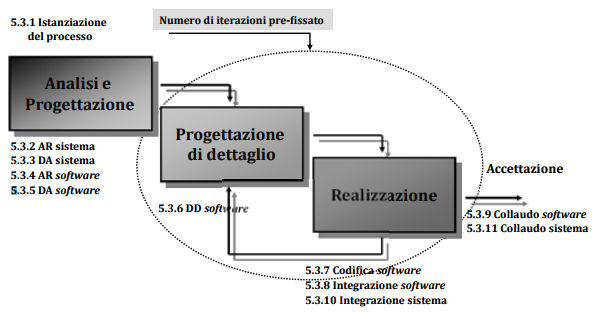
\includegraphics[width=\columnwidth]{sviluppo/ModelloIncrementale} 
    \caption{Modello di ciclo di vita incrementale}
\end{figure}

Tra i principali vantaggi di tale modello vi sono:
\begin{itemize}
	\item ogni incremento di funzionalità permette un avvicinamento alle attese e una riduzione del rischio di fallimento;
	\item le funzionalità più importanti sono le prime a raggiungere la stabilità poiché essendo inserite nei primi incrementi attraversano più cicli di verifica;
	\item il fenomeno del \glossaryItem{big-bang integration} viene evitato producendo valore ad ogni incremento;
	\item il numero di incrementi è fissato in fase di pianificazione.
\end{itemize}

Nello specifico, nella pianificazione del progetto sono stati fissati i seguenti incrementi, tutti corrispondenti ad importanti \glossaryItem{milestone} di progetto:
\begin{enumerate}
	\item realizzazione del servizio web;
	\item realizzazione della logica applicativa;
	\item realizzazione delle interfacce grafiche;
	\item stesura della documentazione annessa al progetto.
\end{enumerate}

Durante il periodo di stage veniva pianificata una riunione con il tutor aziendale al raggiungimento di ogni milestone, al fine verificare che quanto prodotto nella corrispondente baseline fosse inerente alle attese.         % Processi
% !TEX encoding = UTF-8
% !TEX TS-program = pdflatex
% !TEX root = ../tesi.tex

%**************************************************************
\chapter{Background tecnologico} \label{background}
%**************************************************************

In questo capitolo vengono presentate le tecnologie utilizzate durante lo sviluppo di \textit{moviORDER}. La realizzazione dell'applicazione ha permesso l'apprendimento di nuove tecnologie e l'approfondimento di alcune già in parte conosciute. Alcune di queste sono state scelte dallo stagista in seguito al completamento dell'analisi dei requisiti, mentre la maggior parte sono state imposte dal \textit{tutor} aziendale o dal dominio del problema. Le tecnologie scelte dallo stagista sono state concordate con il \textit{team} di sviluppo di \visione{}. Le prossime sezioni presentano le tecnologie in base al contesto in cui sono state utilizzate.

\section{Framework}	

La presentazione delle tecnologie utilizzate per lo sviluppo di \textit{moviORDER} comincia dalla scelta del \textit{framework}, in quanto il \textit{framework} scelto ha imposto l'utilizzo di alcuni linguaggi di programmazione usati durante il periodo di \textit{stage}. Poiché il progetto richiedeva la realizzazione di un'applicazione che funzionasse in ambiente \textit{Android} e \textit{iOS}, il \textit{tutor} aziendale ha consigliato l'utilizzo di un \textit{framework cross-platform}. Questo perché data la diversità delle tecnologie richieste per lo sviluppo di codice nativo \textit{Android} e \textit{iOS}, e la limitata quantità di tempo a disposizione per la realizzazione del progetto, l'utilizzo di un \textit{framework cross-platform} era la migliore soluzione per portare a termine il progetto nei tempi richiesti. Allo stagista è stato richiesto di decidere tra due \glossaryItem{framework cross-platform}: \textit{Xamarin} e \textit{PhoneGap}.\\ Vengono di seguito descritti:
\begin{enumerate}
	\item le motivazioni alla base dei \textit{framework cross-platform};
	\item gli approcci alla base dei \textit{framework cross-platform};
	\item il \textit{framework Xamarin};
	\item il \textit{framework PhoneGap};
	\item le motivazioni che hanno portato \textit{PhoneGap} a prevalere su \textit{Xamarin}.
\end{enumerate}

\subsection{Motivazioni alla base dei framework cross-platform}

Al giorno d'oggi è impensabile realizzare un'applicazione \textit{mobile} per una sola piattaforma perché il mercato è eccessivamente frammentato. Quindi, se si dovesse scegliere di sviluppare un'applicazione per una sola piattaforma si perderebbe una potenziale parte di clienti. La seguente figura mostra, a scopi illustrativi, la frammentazione del mercato italiano nel 2016.

\begin{figure}[!h] 
    \centering 
    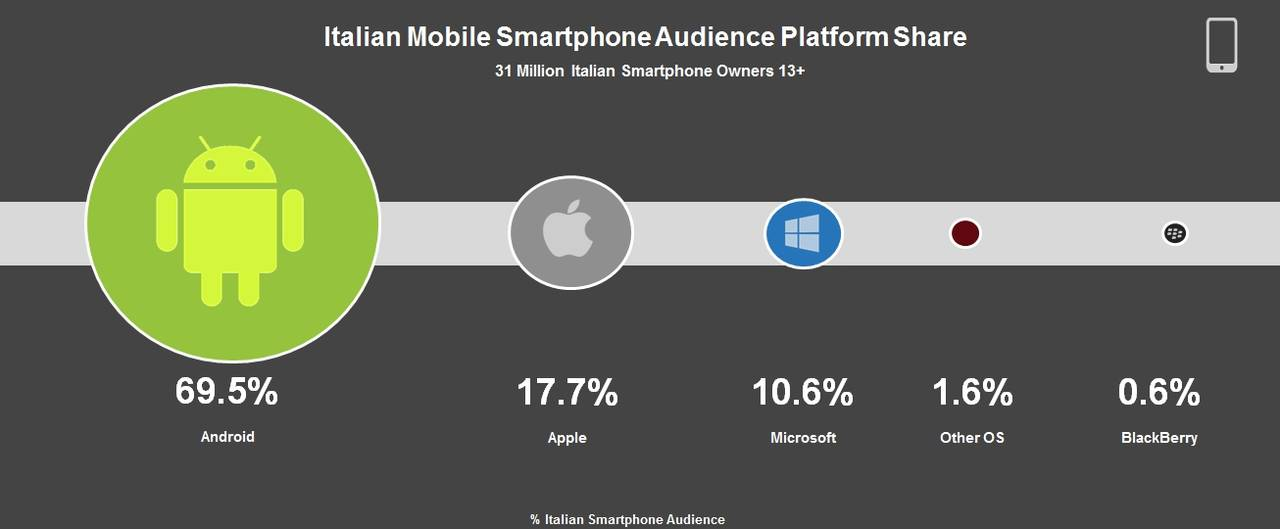
\includegraphics[width=\columnwidth]{tecnologie/mercato} 
    \caption{Frammentazione SO del mercato italiano nel 2016}
\end{figure}

Compresa la necessità di sviluppare più versioni della medesima applicazione in diverse piattaforme, il problema si sposta sulle risorse economiche e sul tempo che si ha a disposizione per lo sviluppo. Infatti sviluppare in diverse piattaforme comporta l'utilizzo di differenti linguaggi di programmazione e quindi la necessità di avere più programmatori esperti, precisamente almeno uno per piattaforma. Altre variabili di cui tener conto sono gli strumenti di sviluppo necessari, le \glossaryItem{API} che si hanno a disposizione e fattori quali i sensori disponibili sui dispositivi, la dimensione degli schermi e le capacità di calcolo differenti.

L'obiettivo dei \textit{framework cross-platform} è la risoluzione di tutti questi problemi in maniera efficiente ed efficace in termini di risorse utilizzate, quindi, più precisamente, la riduzione degli effetti negativi della frammentazione del mercato.

\begin{figure}[!h] 
    \centering 
    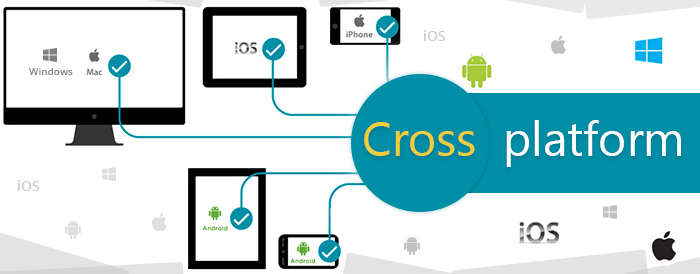
\includegraphics[width=\columnwidth]{tecnologie/framework} 
    \caption{Significato di \textit{cross-platform}}
\end{figure}

Per raggiungere questo obiettivo i \textit{framework cross-platform} consentono di utilizzare un solo linguaggio di programmazione, o un insieme ristretto di linguaggi, per sviluppare un unico codice sorgente, che viene poi convertito nel codice nativo delle piattaforme sulle quali si desidera distribuire l'applicazione. 

Per concludere, dati oggettivi dimostrano che durante il 2016 l'utilizzo dei \textit{framework cross-platform} ha permesso un risparmio in termini di risorse economiche nell'80\% dei casi ed un risparmio di tempo nell'83\% dei casi.

\subsection{Approcci alla base dei framework cross-platform}

Per la scelta del \textit{framework} più idoneo è stato richiesto di studiare gli approcci secondo i quali i \textit{framework} permettono la distribuzione su varie piattaforme. Esistono principalmente quattro approcci in base ai quali è possibile classificare i \textit{framework}:
\begin{itemize}
	\item approccio \textit{web};
	\item approccio ibrido;
	\item approccio interpretato;
	\item approccio \glossaryItem{cross-compiled}.
\end{itemize}

In questa tesi vengono presentati solamente l'approccio ibrido e quello interpretato, poiché utilizzati dai \textit{framework} proposti dal \textit{tutor} aziendale.

L'approccio ibrido si interpone tra la realizzazione di un'applicazione \textit{web} e lo sviluppo di un'applicazione \textit{mobile} in codice nativo. In questo tipo di approccio l'applicazione viene sviluppata utilizzando tecnologie \textit{web} ed eseguita all'interno di un \glossaryItem{container} nativo sul dispositivo \textit{mobile}. Per eseguire l'applicazione viene utilizzato il motore di \textit{rendering} del \textit{browser} del dispositivo, il quale si occupa di interpretare e visualizzare il contenuto \glossaryItem{HTML} (\textit{HyperText Markup Language}) dell'applicazione tramite una visualizzazione \textit{web} a schermo intero. L'accesso alle funzionalità native offerte dal dispositivo è permesso grazie ad un livello astratto che si interpone tra l'applicazione ibrida e tali funzionalità. Questo livello astratto espone le funzionalità tramite \textit{API} \textit{Javascript}. 

\begin{figure}[!h] 
    \centering 
    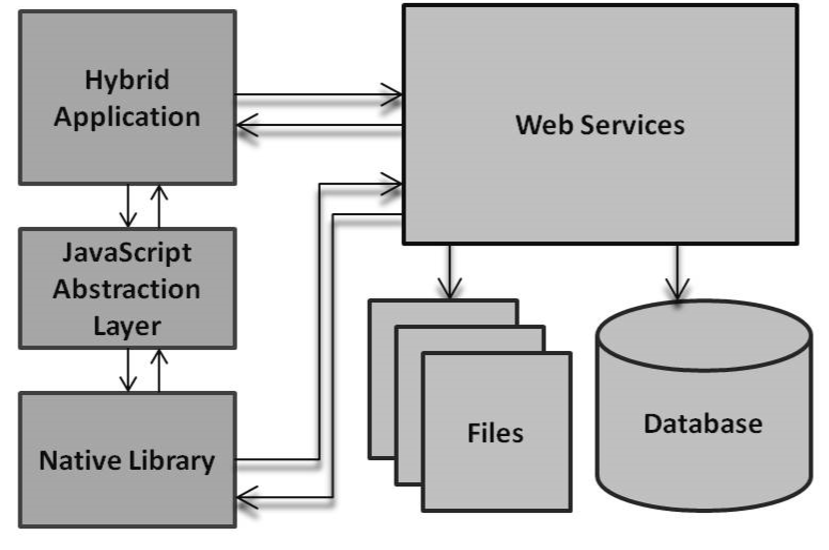
\includegraphics[width=0.9\columnwidth]{tecnologie/ibrido} 
    \caption{Architettura di un'applicazione ibrida}
\end{figure}

\newpage

Nel caso delle applicazioni interpretate il codice sorgente dell'applicazione viene distribuito sul dispositivo \textit{mobile}, dove viene successivamente interpretato da un \glossaryItem{interprete} che si occupa di eseguire il codice a \glossaryItem{run-time}. Lo sviluppo \textit{cross-platform}  è supportato dall'interprete, che permette di eseguire il codice sorgente du differenti piattaforme. L'applicazione interpretata interagisce con un livello astratto per accedere alle \textit{API} native. Un vantaggio di questo approccio è che utilizza elementi delle specifiche interfacce grafiche native per l'interazione utente. Infine, la logica applicativa viene prelevata in maniera del tutto indipendente dalla piattaforma sulla quale l'applicazione viene eseguita.

\begin{figure}[!h] 
    \centering 
    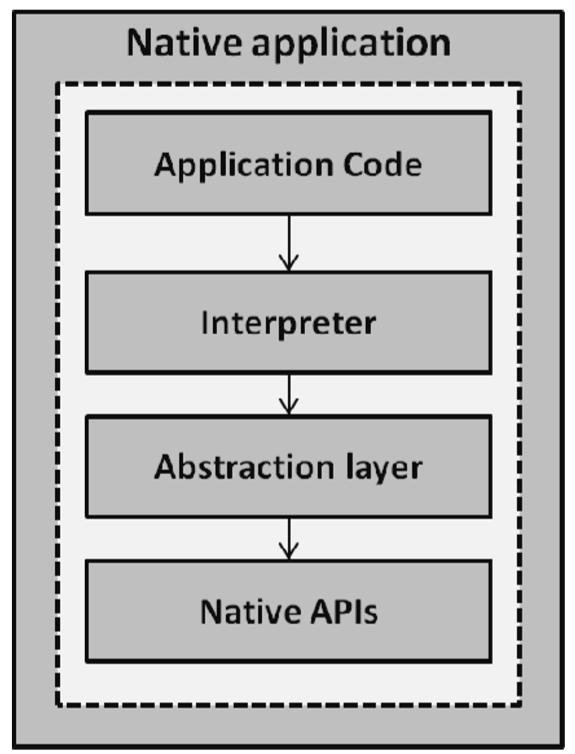
\includegraphics[height=8cm,width=0.6\columnwidth]{tecnologie/interpretato} 
    \caption{Architettura di un'applicazione interpretata}
\end{figure}

\newpage

\subsection{Xamarin}

\textit{Xamarin} è un \textit{framework cross-platform} di proprietà dell'azienda \textit{Microsoft}, il quale utilizza due approcci differenti: l'approccio interpretato per l'ambiente \textit{Android} e \textit{Windows}, e l'approccio \textit{cross-compiled} per l'ambiente \textit{iOS}. Più precisamente, per le piattaforme \textit{Android} e \textit{Windows} è possibile generare l'applicazione direttamente tramite i \textit{tool} messi a disposizione dal \textit{framework} e successivamente distribuirla sui rispettivi \textit{store}, mentre per la piattaforma \textit{iOS} è necessario un passo aggiuntivo. Infatti, per eseguire la compilazione dell'applicazione è richiesto il passaggio per una macchina \textit{Apple} che abbia installato \textit{XCode}. Infine, \textit{Xamarin} richiede che per lo sviluppo dell'applicazione venga utilizzato il linguaggio \glossaryItem{C\#}. Nella figura sottostante viene presentata l'architettura di \textit{Xamarin}.

\begin{figure}[!h] 
    \centering 
    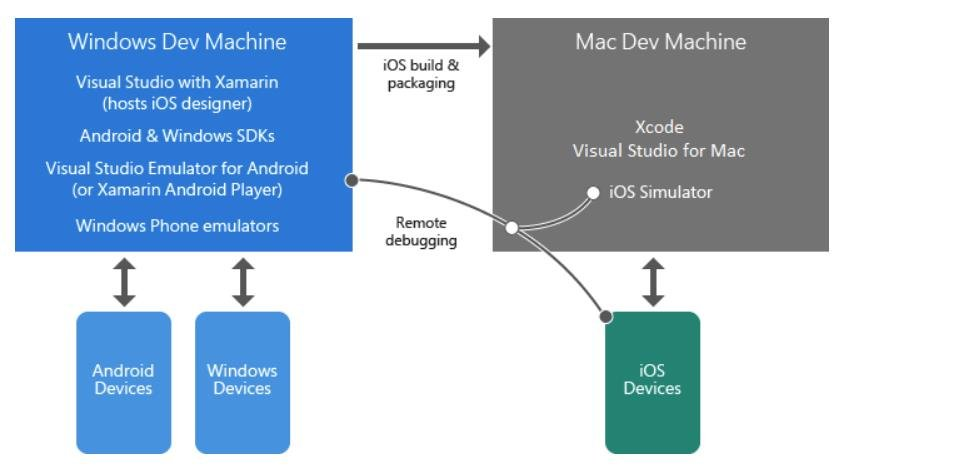
\includegraphics[width=\columnwidth]{tecnologie/xamarinArchitecture} 
    \caption{Architettura del \textit{framework Xamarin}}
\end{figure}

\subsection{PhoneGap}

\textit{PhoneGap} è un \textit{framework cross-platform} di proprietà dell'azienda \textit{Apache}, il quale utilizza un approccio ibrido. Quindi permette la realizzazione di applicazioni \textit{mobile} tramite l'utilizzo di tecnologie \textit{web}, che sono al giorno d'oggi strumenti conosciuti da tutti gli sviluppatori. L'accesso ai componenti \textit{hardware} dei dispositivi \textit{mobile} è permesso grazie all'utilizzo di \glossaryItem{plugin} scaricabili dalla pagina ufficiale del \textit{framework}. Vantaggi importanti del \textit{framework} sono la presenza di documentazione completa per i \textit{plugin} e l'esistenza di una \glossaryItem{community} grande e disponibile. Infine, \textit{PhoneGap} rende disponibili degli strumenti che facilitano lo sviluppo dell'applicazione: \textit{PhoneGap Desktop App}, \textit{PhoneGap CLI}, \textit{PhoneGap App} e \textit{PhoneGap Build}. I primi tre verranno descritti successivamente, in quanto fanno parte dell'ambiente di sviluppo utilizzato durante lo \textit{stage}. \textit{PhoneGap Build} è uno strumento che permette di eseguire la \textit{build} dell'applicazione direttamente su un \textit{server} \textit{cloud Adobe}, a partire da un \textit{file zip} contenente la cartella con il codice sorgente dell'applicazione. In seguito alla \textit{build} è possibile generare e scaricare automaticamente l'applicazione per \textit{Windows} o \textit{Android}. Per \textit{iOS} è necessario fornire i certificati richiesti da \textit{Apple} per la distribuzione dell'applicazione. Nella pagina successiva vengono presentate l'architettura di \textit{PhoneGap} e una figura illustrativa di \textit{PhoneGap Build}.

\begin{figure}[!h] 
    \centering 
    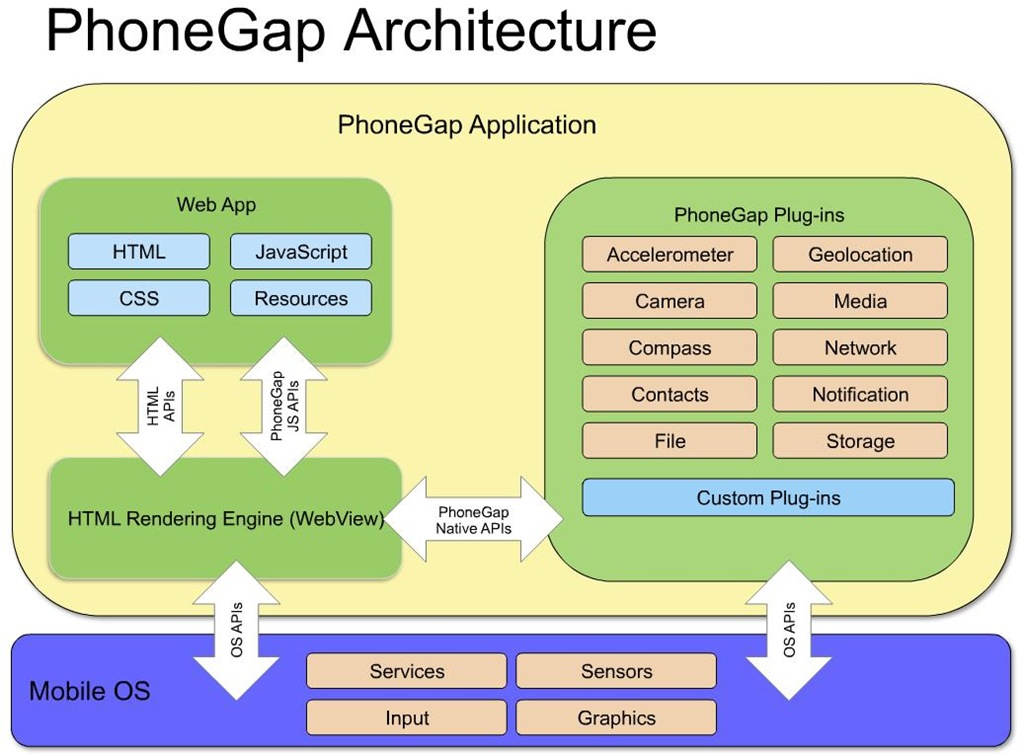
\includegraphics[width=0.9\columnwidth]{tecnologie/phonegapArchitecture} 
    \caption{Architettura del \textit{framework PhoneGap}}
\end{figure}

\begin{figure}[!h] 
    \centering 
    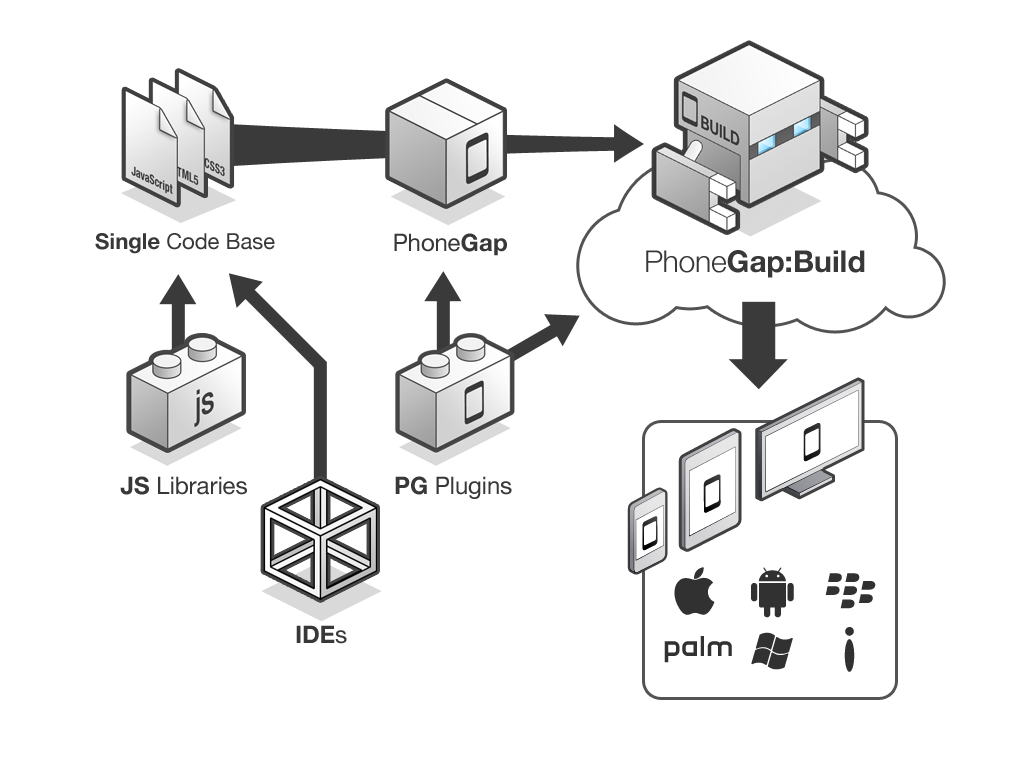
\includegraphics[width=\columnwidth]{tecnologie/phonegapBuild} 
    \caption{Figura illustrativa di \textit{PhoneGap Build}}
\end{figure}

\newpage


\subsection{La scelta di PhoneGap}

I motivi per i quali lo stagista ha optato per il \textit{framework PhoneGap} sono i seguenti:
\begin{enumerate}
	\item \textbf{linguaggio di programmazione}: \textit{PhoneGap} richiedeva l'utilizzo di tecnologie \textit{web} già conosciute e apprese dallo stagista all'Università. Lo studio del linguaggio \textit{C\#} imposto da \textit{Xamarin} avrebbe richiesto un periodo di formazione maggiore delle 40 ore messe a disposizione per lo studio delle tecnologie;
	\item \textbf{linguaggio \textit{Javascript}}: come detto precedentemente, lo stagista era interessato ad approfondire il linguaggio \textit{Javascript}, poiché richiesto al giorno d'oggi dalla maggior parte delle aziende che si occupano della realizzazione di applicazioni \textit{web};
	\item \textbf{facilità nello sviluppo dell'interfaccia grafica}: utilizzando tecnologie \textit{web} risultava semplice progettare e sviluppare un'interfaccia grafica \glossaryItem{responsive}, in grado di adattarsi alla maggior parte dei dispositivi \textit{mobile} presenti sul mercato.
\end{enumerate}

\section{Ambiente di sviluppo}

Durante il periodo di \textit{stage} è stato utilizzato uno specifico ambiente di lavoro, comprendente tecnologie imposte dal \textit{tutor} aziendale e alcune scelte dallo stagista. La qualità delle tecnologie ha impatto diretto sulla qualità di processo e quindi su quella del prodotto, per cui è importante tenere l'ambiente di lavoro costantemente completo, ordinato e aggiornato. Per ottenere questo lo stagista ha dovuto analizzare le tecnologie scelte per assicurarsi che fossero le più adatte per il dominio del problema.

\subsection{Suite di PhoneGap}

La suite di \textit{PhoneGap} ha costituito parte fondamentale dell'ambiente di lavoro. Sono stati utilizzati i seguenti \textit{software}:
\begin{itemize}
	\item \textbf{\textit{PhoneGap Desktop App}}: applicazione utilizzata inizialmente per prendere dimestichezza con il \textit{framework};
	\item \textbf{\textit{PhoneGap CLI}}: interfaccia a linea di comando utilizzata dopo aver preso dimestichezza con il \textit{framework};
	\item \textbf{\textit{PhoneGap App}}: applicazione \textit{mobile} utilizzata inizialmente per testare l'applicazione generata dal \textit{framework}.
\end{itemize}

\textit{PhoneGap Desktop App} è disponibile su \textit{Windows} o \textit{Mac} e permette di iniziare ad utilizzare il \textit{framework} con estrema facilità. Essa fornisce un'interfaccia grafica per creare, gestire e testare progetti \textit{PhoneGap}. Nella pagina successiva viene presentata una figura che mostra l'interfaccia grafica di \textit{PhoneGap Desktop App}.

\begin{figure}[!h] 
    \centering 
    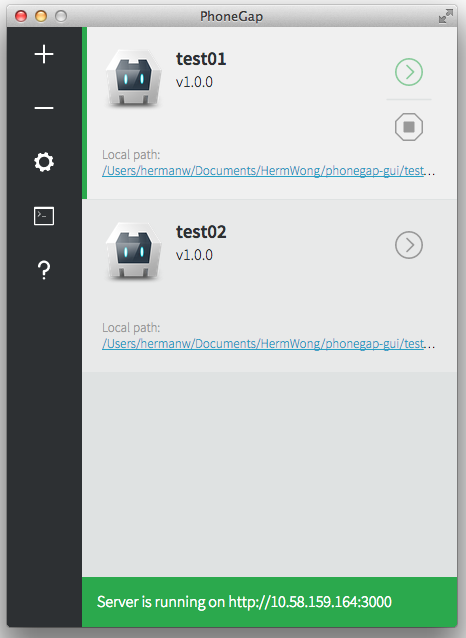
\includegraphics[width=0.8\columnwidth]{tecnologie/phonegapDesktop} 
    \caption{\textit{PhoneGap Desktop App}}
\end{figure}

\newpage

\textit{PhoneGap CLI} estende le funzionalità offerte da \textit{PhoneGap Desktop App} tramite un'interfaccia a riga di comando. Prima del rilascio dell'app desktop, \textit{PhoneGap CLI} veniva utilizzata come strumento principale per configurare e gestire il \textit{framework}. \textit{PhoneGap CLI} può essere utilizzata singolarmente oppure assieme a \textit{PhoneGap Desktop App} e/o \textit{PhoneGap Build}.

\textit{PhoneGap App} è un'applicazione \textit{mobile} che permette di testare l'applicazione \textit{PhoneGap} senza generare ed installare nessun \textit{file} applicazione. Per il test è sufficiente avviare l'esecuzione del progetto su \textit{PhoneGap Desktop App} e collegare il \textit{computer} di sviluppo con il dispositivo su cui è installata \textit{PhoneGap App}. Dopo il collegamento sarà possibile testare completamente l'applicazione.

\begin{figure}[!h] 
    \centering 
    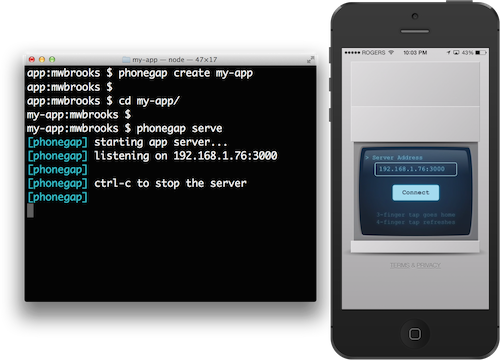
\includegraphics[width=0.8\columnwidth]{tecnologie/phonegapCLIApp} 
    \caption{\textit{PhoneGap CLI} e \textit{PhoneGap App}}
\end{figure}

\subsection{Editor e IDE}

\subsubsection{Sublime Text 3.0}

Per lo sviluppo del progetto \textit{PhoneGap} è stato utilizzato l'\glossaryItem{editor} \textit{Sublime Text 3.0}, ritenuto dallo stagista il più semplice e leggero per la realizzazione di applicazioni \textit{web}. 

\begin{figure}[!h] 
    \centering 
    
\includegraphics[height=4cm,width=4cm]{tecnologie/sublime} 
    \caption{Logo di \textit{Sublime Text 3.0}}
\end{figure}

\subsubsection{Android Studio}

Durante lo \textit{stage} l'applicazione \textit{Android} generata tramite i \textit{tool} offerti dal \textit{framework PhoneGap} non era soddisfacente: spesso non funzionava o l'interfaccia grafica non rispecchiava quella desiderata. Per rendere l'\textit{app} usabile è stato necessario installare \textit{Android Studio}, il quale ha permesso di mettere mano sul codice nativo. \textit{Android Studio} è un ambiente di sviluppo integrato (\glossaryItem{IDE}) basato sul \textit{software} di \textit{JetBrains IntelliJ IDEA} e progettato specificamente per lo sviluppo di applicazioni \textit{Android}.

\begin{figure}[!h] 
    \centering 
    
\includegraphics[height=4.5cm,width=4.5cm]{tecnologie/androidStudio} 
    \caption{Logo di \textit{Android Studio}}
\end{figure}

\subsubsection{XCode}

Durante lo \textit{stage} l'applicazione \textit{iOS} generata tramite i \textit{tool} offerti dal \textit{framework PhoneGap} non era soddisfacente: spesso non funzionava o l'interfaccia grafica non rispecchiava quella desiderata. Per rendere l'\textit{app} usabile è stato necessario installare \textit{XCode}, il quale ha permesso di mettere mano sul codice nativo. \textit{Xcode} è un ambiente di sviluppo integrato (\textit{IDE}), sviluppato e mantenuto da \textit{Apple}, che contiene una suite di strumenti utili allo sviluppo di \textit{software} per i sistemi \textit{macOS}, \textit{iOS}, \textit{watchOS} e \textit{tvOS}.

\begin{figure}[!h] 
    \centering 
    
\includegraphics[height=4cm,width=5cm]{tecnologie/xCode} 
    \caption{Logo di \textit{XCode}}
\end{figure}

\subsubsection{Eclipse JEE}

Durante lo \textit{stage} è stata richiesta la realizzazione di un servizio \textit{web} che si interponesse tra la logica applicativa di \textit{moviORDER} e un \textit{database} presente sul \textit{server Azure} di \visione{}. Il servizio \textit{web} è stato realizzato in linguaggio \textit{Java} tramite l'utilizzo di oggetti \textit{servlet}. Per lo sviluppo degli oggetti \textit{servlet} è stato utilizzato l'\textit{IDE Eclipse JEE}, il quale offre buoni strumenti per lo sviluppo di applicazioni \textit{web} \textit{Java}. \textit{Eclipse} è un ambiente di sviluppo integrato multi-linguaggio e multipiattaforma, ideato da un consorzio di grandi società quali \textit{Ericsson}, \textit{HP}, \textit{IBM}, \textit{Intel}, \textit{MontaVista Software}, \textit{QNX}, \textit{SAP} e \textit{Serena Software}, chiamato \textit{Eclipse Foundation}.

\begin{figure}[!h] 
    \centering 
    
\includegraphics[width=0.8\columnwidth]{tecnologie/eclipse} 
    \caption{Logo di \textit{Eclipse}}
\end{figure}

\newpage

\subsection{Gestione DBMS}

Durante il progetto è stato utilizzato il \glossaryItem{DBMS} \textit{Microsoft SQL Server} per gestire il \textit{database} di \textit{moviORDER}. Per una gestione veloce ed ottimale dello stesso si è deciso di usare il \textit{software} \textit{SQL Server Management Studio}. \textit{SQL Server Management Studio} (\textit{SSMS}) è un'applicazione \textit{software} usata per configurare, gestire e amministrare \textit{database}, in locale o su un \textit{server cloud}, con il \textit{DBMS Microsoft SQL Server}. 

\begin{figure}[!h] 
    \centering 
    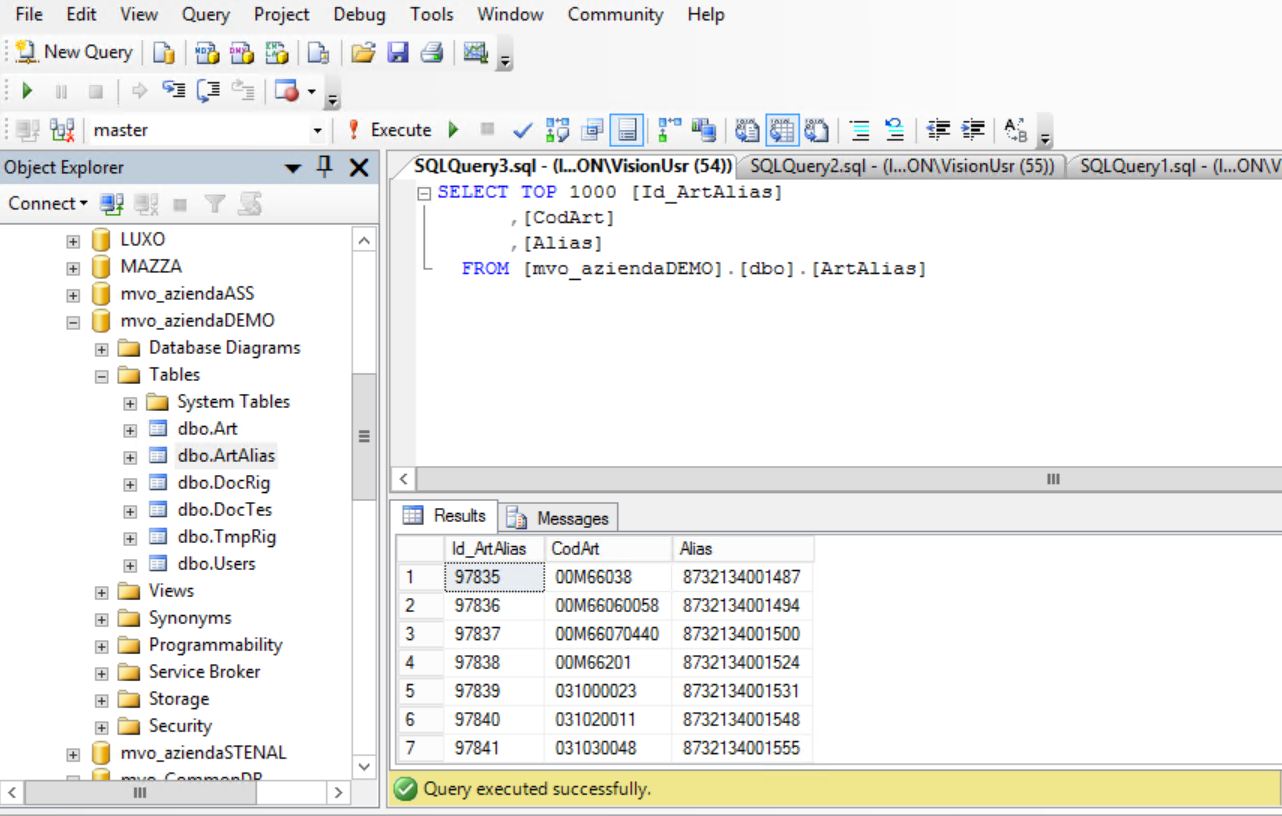
\includegraphics[width=\columnwidth]{tecnologie/ssms} 
    \caption{\textit{Screenshot} di \textit{SQL Server Management Studio}}
\end{figure}

\newpage

\subsection{Server web}

Per permettere l'esecuzione del servizio \textit{web} sul \textit{server cloud} di \visione{} si è utilizzato \textit{Apache Tomcat}. \textit{Apache Tomcat} (o semplicemente \textit{Tomcat}) è un \glossaryItem{server web} (nella forma di contenitore \textit{servlet}) \textit{open source} sviluppato dalla \textit{Apache Software Foundation}. Implementa le specifiche \glossaryItem{JavaServer Pages} (\textit{JSP}) e \textit{servlet}, fornendo quindi una piattaforma \textit{software} per l'esecuzione di applicazioni \textit{web} sviluppate in linguaggio \textit{Java}.

\begin{figure}[!h] 
    \centering 
    
\includegraphics[height=4cm,width=5cm]{tecnologie/tomcat} 
    \caption{Logo di \textit{Apache Tomcat}}
\end{figure}

\subsection{Cloud computing}

Il servizio \textit{web} e il \textit{database} con il quale l'applicazione interagisce risiedono su un \textit{server Azure} di \visione{}. \textit{Microsoft Azure} (precedentemente nota come \textit{Windows Azure}) è la piattaforma \textit{cloud} pubblica di \textit{Microsoft}, che offre servizi di \glossaryItem{cloud computing}. Tramite Azure vengono erogati servizi appartenenti a diverse categorie, quali: risorse di elaborazione, archiviazione e memorizzazione dati, trasmissione dati e interconnessione di reti, analisi, \textit{intelligence}, apprendimento automatico, sicurezza e gestione delle identità, monitoraggio e gestione, nonché servizi per lo sviluppo di applicazioni. Per accedere al \textit{server} da remoto è stato utilizzato il \textit{software} ``Connessione \textit{Desktop} Remoto di \textit{Windows}''.

\begin{figure}[!h] 
    \centering 
    
\includegraphics[width=0.8\columnwidth]{tecnologie/azure} 
    \caption{Logo di \textit{Microsoft Azure}}
\end{figure}

\newpage

\subsection{Strumenti di testing}

Durante lo sviluppo di \textit{moviORDER} sono stati eseguiti dei test per verificare il corretto funzionamento del servizio \textit{web} e dell'applicazione. Per il test dell'\textit{API} del servizio \textit{web} si è utilizzato \textit{Postman}. \textit{Postman} è uno strumento di \glossaryItem{API testing} che permette di testare \textit{API} direttamente, o come parte di test d'integrazione, per determinare se soddisfano criteri di funzionalità, affidabilità, performance e sicurezza. Nel caso di \textit{moviORDER}, il test avviene tramite l'invio di una richiesta \textit{HTTP POST} all'\textit{API} sul \textit{server cloud}. Successivamente il \textit{software} visualizza la stringa in formato \textit{JSON} restituita dal \textit{server} e lo sviluppatore può verificare se la risposta del servizio è quella attesa.

\begin{figure}[!h] 
    \centering 
    
\includegraphics[height=4cm,width=5cm]{tecnologie/postman} 
    \caption{Logo di \textit{Postman}}
\end{figure}

Per testare il corretto funzionamento dell'applicazione si è utilizzata la \textit{console} del \textit{browser Google Chrome}, facente parte degli strumenti offerti dallo stesso per gli sviluppatori \textit{web}. Tramite la \textit{console} è stato possibile verificare il codice \textit{JavaScript} che costituisce la logica applicativa di \textit{moviORDER}.

\begin{figure}[!h] 
    \centering 
    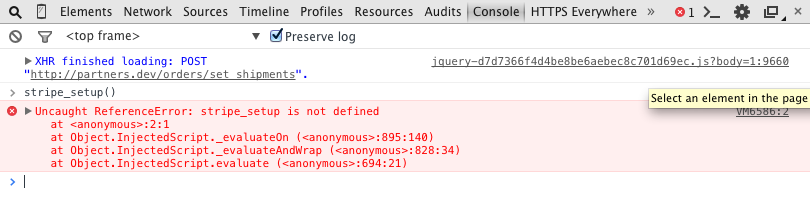
\includegraphics[width=\columnwidth]{tecnologie/console} 
    \caption{\textit{Screenshot} della console di \textit{Google Chrome}}
\end{figure}

\newpage

\subsection{Strumenti di versioning e ticketing}

Per scelta dello stagista il progetto è stato sottoposto a controllo di versione in ogni sua parte: applicazione, servizio \textit{web} e documentazione. Questo ha permesso, principalmente nel caso dell'applicazione, di tornare a \glossaryItem{baseline} sicure nel caso di sovrascritture, perdite accidentali e \glossaryItem{commit} di codice con errori di programmazione. Per il controllo di versione si è utilizzato lo strumento \textit{Git} e in particolare il servizio di hosting \textit{GitHub}. Lo stagista ha scelto tali \textit{software} poiché già utilizzati in progetti didattici durante l'Università.

\begin{figure}[!h] 
    \centering 
    
\includegraphics[height=5cm,width=5cm]{tecnologie/git} 
    \caption{Logo di \textit{GitHub}}
\end{figure}

Lo stagista ha scelto inoltre di utilizzare lo strumento di \glossaryItem{ticketing} \textit{Asana}, in modo da facilitare la pianificazione del progetto. \textit{Asana} è un'applicazione \textit{web} e \textit{mobile} progettata per aiutare i \textit{team} ad organizzare, tracciare e gestire il loro lavoro. In particolare, lo strumento è stato utilizzato per dare una scadenza ai \textit{task} assegnati dal \textit{tutor} aziendale.

\begin{figure}[!h] 
    \centering 
    
\includegraphics[height=5cm,width=7cm]{tecnologie/asana} 
    \caption{Logo di \textit{Asana}}
\end{figure}

\subsection{Strumenti di modellazione e documentazione}

Il progetto ha richiesto lo sviluppo di diagrammi di \textit{Gantt} in fase di pianificazione e di diagrammi \glossaryItem{UML} (\textit{Unified Modeling Language}) in fase di analisi dei requisiti e progettazione. Per la realizzazione dei diagrammi di \textit{Gantt} si è utilizzato \textit{Gantt Project}, per i diagrammi \textit{UML} dei casi d'uso si è utilizzato \textit{Astah UML}, mentre per i diagrammi \textit{UML} dei \textit{package} e delle classi si è utilizzato \textit{Visual Paradigm CE}. I \textit{software} sono stati scelti perché già appresi durante il progetto di Ingegneria del \textit{Software} all'Università.

\begin{figure}[!h] 
    \centering 
    	\subfloat{
\includegraphics[width=0.33\columnwidth]{tecnologie/gantt}}
    	\subfloat{
\includegraphics[width=0.33\columnwidth]{tecnologie/astah}} 
    	\subfloat{
\includegraphics[width=0.33\columnwidth]{tecnologie/vp}} 
    \caption{Loghi di \textit{Gantt Project}, \textit{Astah UML} e \textit{Visual Paradigm CE}}
\end{figure}

Per la realizzazione dei diagrammi \glossaryItem{ER} (\textit{Entity Relationship}) e delle figure illustrative dell'architettura del prodotto si è utilizzato il \textit{software} \textit{Lucidchart}. Per la stesura della documentazione si è utilizzato l'\textit{editor} \textit{TexMaker}, anch'esso appreso durante il progetto di Ingegneria del \textit{Software}. \textit{TexMaker} permette l'integrazione con un dizionario per il controllo ortografico e la compilazione e visione del \textit{pdf} prodotto.

\begin{figure}[!h] 
    \centering 
    \subfloat{
\includegraphics[height=4.5cm,width=4.5cm]{tecnologie/lucid}}
    \subfloat{
\includegraphics[height=4.5cm,width=4.5cm]{tecnologie/tex}}
    \caption{Loghi di \textit{Lucidchart} e \textit{TexMaker}}
\end{figure}

\subsection{Linguaggi di programmazione e murkup}

\subsubsection{HTML5, CSS3 e JavaScript}

Siccome è stato scelto il \textit{framework PhoneGap}, lo stagista ha dovuto utilizzare i linguaggi \textit{HTML5}, \glossaryItem{CSS3} e \textit{JavaScript}, in quanto \textit{PhoneGap} richiede di sviluppare l'applicazione tramite l'utilizzo di tecnologie \textit{web}. In particolare, \textit{HTML5} è stato scelto perché include un insieme di funzionalità che permettono di valorizzare le interfacce \textit{mobile}. Alcune di queste evidenziano come \textit{HTML5} sia già per sua natura orientato al \textit{mobile}. In particolare \textit{HTML5} fornisce \textit{API} per:
\begin{itemize}
	\item \textbf{geolocalizzazione}: con la scrittura di poco codice, forniscono la posizione del dispositivo in coordinate terrestri. Quindi, la stessa funzionalità su uno \textit{smartphone} o un \textit{tablet} fornisce la posizione dell'utente stesso;
	\item \textbf{eventi \textit{touch}}: mentre i meccanismi di input nei PC consistono per lo più nella tastiera e nel mouse, nei dispositivi mobili quasi tutto passa per il \textit{touch screen}, e avere funzionalità comode per gestire questo strumento consente un'interazione più ricca e senza limitazioni per l'utente. Le gestualità da attuare su un \textit{display}, nel mondo \textit{mobile}, costituiscono un vero e proprio linguaggio fondamentale nella \textit{user experience};
	\item \textbf{controllo batteria}: considerata l'importanza rivestita dalle risorse energetiche, l'esistenza stessa di questa libreria nel linguaggio dimostra come il suo impiego sia particolarmente mirato al panorama \textit{mobile}.
\end{itemize}

Ciò che ha favorito la scelta di \textit{CSS3} sono state le \glossaryItem{media queries}. Esse permettono di definire regole stilistiche in base alla tipologia del mezzo di visualizzazione, delle sue dimensioni e della sua attuale disposizione (\textit{portrait} o \textit{landscape}). Ciò influisce non solo sull'aspetto esteriore degli elementi ma anche sul loro posizionamento e quindi sulla struttura stessa dell'interfaccia.

Per quanto riguarda il linguaggio \textit{JavaScript} si è utilizzato \textit{JavaScript} puro, senza l'utilizzo di \textit{framework} o \glossaryItem{JQuery}. Una particolarità del linguaggio, detta \textit{AJAX}, ha reso possibile eseguire chiamate all'\textit{API} del servizio \textit{web} di \textit{moviORDER}. \textit{AJAX}, acronimo di \textit{\textit{Asynchronous JavaScript and XML}}, è una tecnica di sviluppo \textit{software} per la realizzazione di applicazioni \textit{web} interattive (\textit{Rich Internet Application}). Lo sviluppo di applicazioni \textit{HTML} con \textit{AJAX} si basa su uno scambio di dati in \textit{background} fra \textit{web browser} e \textit{server}, che consente l'aggiornamento dinamico di una pagina \textit{web} senza esplicito ricaricamento da parte dell'utente.

\begin{figure}[!h] 
    \centering 
    	
\includegraphics[width=0.8\columnwidth]{tecnologie/html5}
    \caption{Loghi di \textit{HTML5}, \textit{CSS3} e \textit{JavaScript}}
\end{figure}

I linguaggi scelti, grazie alle loro caratteristiche che li rendono orientati allo sviluppo \textit{mobile}, insieme ai meccanismi che il \textit{framework PhoneGap} utilizza per convertire una \textit{web application} in un'applicazione \textit{mobile}, permettono di effettuare meno modifiche in seguito per perfezionare l'applicazione su \textit{Android} e \textit{iOS}.

\subsubsection{Java}

Per la realizzazione del servizio \textit{web} si è utilizzato il linguaggio \textit{Java}. La scelta poteva ricadere su \textit{Java} o \glossaryItem{PHP} (\textit{HyperText Preprocessor}). È stato scelto \textit{Java} in quanto possiede un compilatore, risulta più facilmente ``\textit{debuggabile}'' rispetto a \textit{PHP} e permette l'utilizzo di oggetti \textit{servlet}. I \textit{servlet} sono oggetti \textit{Java} che operano all'interno di un \textit{server web}, oppure un \textit{server} per applicazioni, che permettono la creazione di un'applicazione \textit{web}. Nel caso del progetto, i \textit{servlet} hanno permesso lo sviluppo dell'\textit{API} che costituisce il servizio \textit{web}. Una descrizione dell'\textit{API}, di come i \textit{servlet} sono stati utilizzati nel progetto e di come l'\textit{API} viene interrogata dall'applicazione, è presente in sezione §\ref{api}.

\begin{figure}[!h] 
    \centering 
    
\includegraphics[height=4.5cm,width=4.5cm]{tecnologie/java} 
    \caption{Logo di \textit{Java}}
\end{figure}

\subsubsection{\LaTeX{}}

Per la stesura della documentazione annessa a \textit{moviORDER} è stato utilizzato il linguaggio \LaTeX{}. La scelta è ricaduta su \LaTeX{} poiché già appreso e utilizzato durante il progetto di Ingegneria del \textit{Software}. \LaTeX{} è un linguaggio di \textit{markup} usato per la preparazione di testi, basato sul programma di composizione tipografica \TeX{}. Fornisce funzioni di \glossaryItem{desktop publishing} programmabili e mezzi per l'automazione della composizione tipografica, inclusa la numerazione, i riferimenti incrociati, tabelle e figure, organizzazione delle pagine, bibliografie e molto altro. Infine la particolarità più utile del linguaggio è l'esistenza di \textit{community} che rendono disponibili \glossaryItem{template} riutilizzabili, come quello che è stato utilizzato per la stesura di questa tesi.

\begin{figure}[!h] 
    \centering 
    
\includegraphics[height=3cm,width=6cm]{tecnologie/latex} 
    \caption{Logo di \LaTeX{}}
\end{figure}

\subsection{DBMS}

Per la creazione, gestione e amministrazione di \textit{database} è stato utilizzato il \textit{DBMS Microsoft SQL Server}. È stato scelto questo \textit{software} poiché già ampiamente utilizzato all'interno di \visione{}. In questo modo gli sviluppatori dell'azienda potranno occuparsi della manutenzione del \textit{database} di \textit{moviORDER} con un \textit{DBMS} conosciuto. \textit{Microsoft SQL Server} usa una variante del linguaggio \glossaryItem{SQL} (\textit{Structured Query Language}) standard chiamata \glossaryItem{Transact-SQL} (\textit{T-SQL}). \textit{Transact-SQL} espande le prestazioni di \textit{SQL} aggiungendo:
\begin{itemize}
	\item funzioni per controllo di flusso;
	\item possibilità di definire variabili locali;
	\item varie funzioni per la manipolazione di stringhe, date ed espressioni matematiche;
	\item miglioramento delle istruzioni \textit{DELETE} e \textit{UPDATE}.
\end{itemize}

\begin{figure}[!h] 
    \centering 
    
\includegraphics[height=5cm,width=7cm]{tecnologie/sqlserver} 
    \caption{Logo di \textit{SQL Server}}
\end{figure}    % Kick-Off
% !TEX encoding = UTF-8
% !TEX TS-program = pdflatex
% !TEX root = ../tesi.tex

%**************************************************************
\chapter{Analisi dei requisiti}
\label{cap:analisi-requisiti}
%**************************************************************

Questo capitolo descrive i casi d'uso e i requisiti della piattaforma moviORDER, individuati e classificati per definire nel dettaglio obiettivi e funzionalità del sistema. I casi d'uso e i requisiti sono stati dedotti da un'analisi preliminare eseguita dal tutor aziendale, la quale è stata perfezionata dallo stagista per perseguire massima efficienza ed efficacia del sistema. Le convenzioni adottate per la stesura di casi d'uso e requisiti sono presenti in Appendice §\ref{}.

\section{Casi d'uso}

Per lo studio dei casi di utilizzo della piattaforma sono stati creati dei diagrammi dei casi d'uso che meglio descrivono funzioni e/o servizi offerti dal sistema, così come sono percepiti e utilizzati dagli attori che interagiscono con il sistema stesso. Per la definizione dei diagrammi UML dei casi d'uso è stato utilizzato lo standard UML 2.0.

\subsection{Attori del sistema}

Lo scopo di moviORDER è permettere alle aziende che forniscono dei prodotti di vendere gli stessi ai propri clienti tramite un'applicazione multipiattaforma. Quindi moviORDER viene distribuita da VISIONEIMPRESA alle aziende che forniscono prodotti, la quale viene distribuita dalle aziende stesse ai propri clienti. Gli utilizzatori finali di moviORDER sono quindi i clienti delle singole aziende che sono clienti di VISIONEIMPRESA.
L'accesso all'applicazione è consentito solamente agli utenti provvisti di credenziali di accesso, le quali vengono distribuite, insieme all'applicazione, dal fornitore. Non è prevista quindi una funzionalità di registrazione. Nel contesto di moviORDER vi sono quindi due tipologie di attori:
\begin{enumerate}
	\item \textbf{Utente non autenticato}: è un utente che non ha effettuato l'accesso al sistema al quale viene offerta la sola funzionalità di autenticazione. Una volta che un utente non autenticato viene riconosciuto accedendo al sistema, diventa un utente autenticato;
	\item \textbf{Utente autenticato}: è un utente che ha effettuato l'accesso al sistema e che può usufruire di tutte le sue funzionalità. Le funzionalità offerte all'utente autenticato sono:
	\begin{itemize}
		\item possibilità di effettuare il logout;
		\item possibilità di aggiungere articoli al proprio carrello;
		\item possibilità di modificare gli articoli nel proprio carrello;
		\item possibilità di rimuovere articoli dal proprio carrello;
		\item possibilità di inviare un ordine alla propria azienda.
	\end{itemize}
\end{enumerate}

\subsection{UC1 - Azioni utente non autenticato}

\begin{figure}[!h] 
    \centering 
    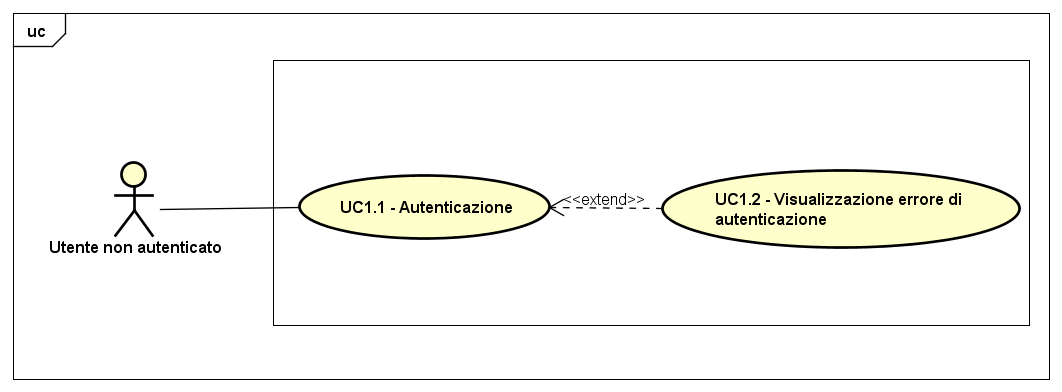
\includegraphics[width=0.9\columnwidth]{usecase/generaleNonAutenticato} 
    \caption{Use Case - UC1: Azioni utente non autenticato}
\end{figure}

\begin{itemize}
	\item \textbf{Attore}: Utente non autenticato;
	\item \textbf{Descrizione}: L'attore può eseguire l'operazione di autenticazione alla piattaforma moviORDER;
	\item \textbf{Pre-condizioni}: L'attore ha avviato l'applicazione, possiede le credenziali di accesso e non è ancora stato riconosciuto dal sistema;
	\item \textbf{Post-condizioni}: L'attore ha eseguito l'operazione di autenticazione;
	\item \textbf{Scenario principale}: UC1.1 - Autenticazione;
	\item \textbf{Scenario alternativo}: L'attore ha fornito credenziali di accesso non corrispondenti a nessun utente registrato dall'azienda, oppure non riesce ad accedere al sistema perché è stato bloccato dall'azienda stessa: UC1.2 - Visualizzazione errore di autenticazione. 
\end{itemize}

\subsection{UC1.1 - Autenticazione}

\begin{figure}[!h] 
    \centering 
    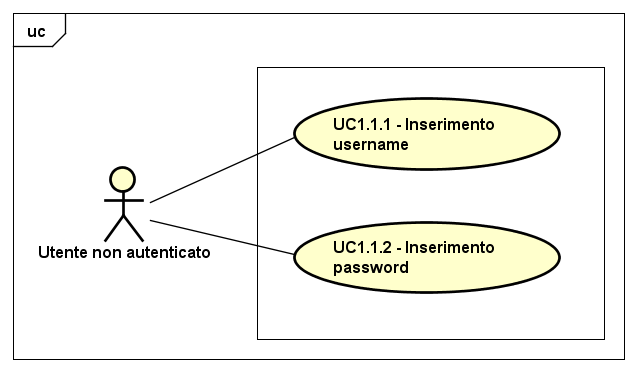
\includegraphics[width=0.9\columnwidth]{usecase/autenticazione} 
    \caption{Use Case - UC1.1: Autenticazione}
\end{figure}

\begin{itemize}
	\item \textbf{Attore}: Utente non autenticato;
	\item \textbf{Descrizione}: L'attore può eseguire l'operazione di autenticazione;
	\item \textbf{Pre-condizioni}: L’attore ha avviato l’applicazione, non è ancora riconosciuto dal sistema ed ha espresso la volontà di effettuare l’autenticazione a moviORDER;
	\item \textbf{Post-condizioni}: L’attore ha eseguito l’operazione di accesso al sistema ed è quindi ora riconosciuto come utente autenticato;
	\item \textbf{Scenario principale}: 
		\begin{enumerate}
			\item UC1.1.1 - Inserimento username;
			\item UC1.1.2 - Inserimento password.
		\end{enumerate} 
\end{itemize}

\subsection{UC2 - Azioni utente autenticato}

\begin{figure}[!h] 
    \centering 
    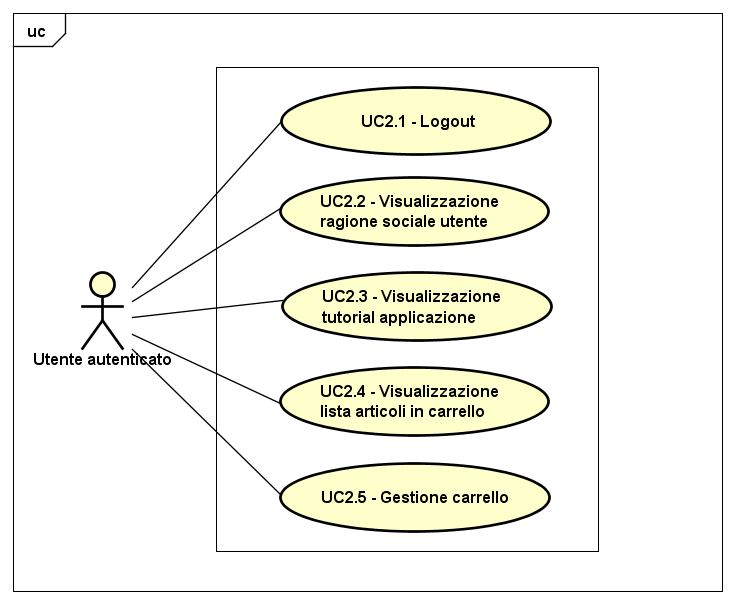
\includegraphics[width=0.9\columnwidth]{usecase/generaleAutenticato} 
    \caption{UC2 - Azioni utente autenticato}
    \label{fig:altoLivello2}
\end{figure}

\begin{itemize}
	\item \textbf{Attore}: Utente autenticato;
	\item \textbf{Descrizione}: L'attore può:
	\begin{enumerate}
		\item Eseguire l'operazione di logout;
		\item Visualizzare la propria ragione sociale;
		\item Visualizzare il tutorial dell'applicazione premendo sul relativo bottone;
		\item Visualizzare la lista degli articoli in carrello;
		\item Gestire il proprio carrello. 
	\end{enumerate}
	\item \textbf{Pre-condizioni}: L'attore è stato riconosciuto dal sistema;
	\item \textbf{Post-condizioni}: L'attore ha eseguito le azioni che desiderava compiere all'interno del sistema;
	\item \textbf{Scenario principale}: 
		\begin{enumerate}
			\item UC2.1 - Logout;
			\item UC2.2 - Visualizzazione ragione sociale utente;
			\item UC2.3 - Visualizzazione tutorial applicazione;
			\item UC2.4 - Visualizzazione lista articoli in carrello;
			\item UC2.5 - Gestione carrello.
		\end{enumerate}
\end{itemize}

\subsection{UC2.4 - Visualizzazione lista articoli in carrello}

\subsection{UC2.4.1 - Visualizzazione singolo articolo in carrello}

\subsection{UC2.5 - Gestione carrello}

\subsection{UC2.5.1 - Aggiunta articolo}

\subsection{UC2.5.2 - Modifica articolo}

\subsection{UC2.5.11 - Invio ordine}

\section{Tracciamento dei requisiti}

Da un'attenta analisi dei requisiti e degli use case effettuata sul progetto è stata stilata la tabella che traccia i requisiti in rapporto agli use case.\\
Sono stati individuati diversi tipi di requisiti e si è quindi fatto utilizzo di un codice identificativo per distinguerli.\\
Il codice dei requisiti è così strutturato R(F/Q/V)(N/D/O) dove:
\begin{enumerate}
	\item[R =] requisito
    \item[F =] funzionale
    \item[Q =] qualitativo
    \item[V =] di vincolo
    \item[N =] obbligatorio (necessario)
    \item[D =] desiderabile
    \item[Z =] opzionale
\end{enumerate}
Nelle tabelle \ref{tab:requisiti-funzionali}, \ref{tab:requisiti-qualitativi} e \ref{tab:requisiti-vincolo} sono riassunti i requisiti e il loro tracciamento con gli use case delineati in fase di analisi.

\newpage

\begin{table}%
\caption{Tabella del tracciamento dei requisti funzionali}
\label{tab:requisiti-funzionali}
\begin{tabularx}{\textwidth}{lXl}
\hline\hline
\textbf{Requisito} & \textbf{Descrizione} & \textbf{Use Case}\\
\hline
RFN-1     & L'interfaccia permette di configurare il tipo di sonde del test & UC1 \\
\hline
\end{tabularx}
\end{table}%

\begin{table}%
\caption{Tabella del tracciamento dei requisiti qualitativi}
\label{tab:requisiti-qualitativi}
\begin{tabularx}{\textwidth}{lXl}
\hline\hline
\textbf{Requisito} & \textbf{Descrizione} & \textbf{Use Case}\\
\hline
RQD-1    & Le prestazioni del simulatore hardware deve garantire la giusta esecuzione dei test e non la generazione di falsi negativi & - \\
\hline
\end{tabularx}
\end{table}%

\begin{table}%
\caption{Tabella del tracciamento dei requisiti di vincolo}
\label{tab:requisiti-vincolo}
\begin{tabularx}{\textwidth}{lXl}
\hline\hline
\textbf{Requisito} & \textbf{Descrizione} & \textbf{Use Case}\\
\hline
RVO-1    & La libreria per l'esecuzione dei test automatici deve essere riutilizzabile & - \\
\hline
\end{tabularx}
\end{table}%         % Concept Preview
% !TEX encoding = UTF-8
% !TEX TS-program = pdflatex
% !TEX root = ../tesi.tex

%**************************************************************
\chapter{Progettazione e codifica}
\label{cap:progettazione-codifica}
%**************************************************************

\intro{Breve introduzione al capitolo}\\

%**************************************************************
\section{Tecnologie e strumenti}
\label{sec:tecnologie-strumenti}

Di seguito viene data una panoramica delle tecnologie e strumenti utilizzati.

\subsection*{Tecnologia 1}
Descrizione Tecnologia 1.

\subsection*{Tecnologia 2}
Descrizione Tecnologia 2

%**************************************************************
\section{Ciclo di vita del software}
\label{sec:ciclo-vita-software}

%**************************************************************
\section{Progettazione}
\label{sec:progettazione}

\subsubsection{Namespace 1} %**************************
Descrizione namespace 1.

\begin{namespacedesc}
    \classdesc{Classe 1}{Descrizione classe 1}
    \classdesc{Classe 2}{Descrizione classe 2}
\end{namespacedesc}


%**************************************************************
\section{Design Pattern utilizzati}

%**************************************************************
\section{Codifica}
               % Product Prototype
% !TEX encoding = UTF-8
% !TEX TS-program = pdflatex
% !TEX root = ../tesi.tex

%**************************************************************
\chapter{Verifica e validazione}
\label{cap:verifica-validazione}
%**************************************************************               % Product Design Freeze e SOP
% !TEX encoding = UTF-8
% !TEX TS-program = pdflatex
% !TEX root = ../tesi.tex

%**************************************************************
\chapter{Conclusioni}
\label{cap:conclusioni}
%**************************************************************

%**************************************************************
\section{Consuntivo finale}

%**************************************************************
\section{Raggiungimento degli obiettivi}

%**************************************************************
\section{Conoscenze acquisite}

%**************************************************************
\section{Valutazione personale}
               % Conclusioni
\appendix     
\chapter{Convenzioni} \label{convenzioni}

In questo capitolo vengono presentate le convenzioni utilizzate per la classificazione di casi d'uso e requisiti.

\section{Casi d'uso}

Ogni caso d'uso è classificato tramite il seguente formalismo:
\begin{center}
	\textbf{UC$\{$codice\_identificativo$\}$}
\end{center}

dove:

\begin{itemize}
	\item \textbf{codice\_identificativo}: è un codice composto da una serie di numeri separati tramite punto, che identificano il caso d'uso in maniera univoca e lo esprimono gerarchicamente.
\end{itemize}

\section{Requisiti}

Ogni requisito è classificato tramite il seguente formalismo:
\begin{center}
	\textbf{R$\{$X$\}$$\{$Y$\}$$\{$codice\_identificativo$\}$}
\end{center}

dove:

\begin{itemize}
	\item \textbf{X} specifica la tipologia di requisito:
        \begin{itemize}
            \item \textit{F}: requisito funzionale;
            \item \textit{Q}: requisito qualitativo;
            \item \textit{V}: requisito di vincolo.
        \end{itemize}
    \item \textbf{Y} indica uno dei seguenti gradi di necessità:
        \begin{itemize}
            \item \textit{O}: requisito obbligatorio;
            \item \textit{D}: requisito desiderabile;
            \item \textit{F}: requisito facoltativo.
        \end{itemize}
    \item \textbf{codice\_identificativo}: è un codice composto da una serie di numeri separati tramite
    punto, che identificano il requisito in maniera univoca e lo esprimono gerarchicamente.
\end{itemize}    
                          
% !TEX encoding = UTF-8
% !TEX TS-program = pdflatex
% !TEX root = ../tesi.tex

%**************************************************************
\chapter{Appendice A}
%**************************************************************

\epigraph{Citazione}{Autore della citazione}



               % Appendice A

%**************************************************************
% Materiale finale
%**************************************************************
\backmatter
\printglossaries
% !TEX encoding = UTF-8
% !TEX TS-program = pdflatex
% !TEX root = ../tesi.tex

%**************************************************************
% Bibliografia
%**************************************************************

\cleardoublepage
\chapter{Bibliografia}

\begin{enumerate}[label={[\arabic*]}]
	\item \textit{Agile, definizione} - \url{https://en.wikipedia.org/wiki/Agile_software_development}
	\item \textit{AJAX, definizione} - \url{https://en.wikipedia.org/wiki/Ajax_(programming)}
	\item \textit{API, definizione} - \url{https://en.wikipedia.org/wiki/Application_programming_interface}
	\item \textit{API testing, definizione} - \url{https://en.wikipedia.org/wiki/API_testing}
	\item \textit{Applicazione web, definizione} - \url{https://en.wikipedia.org/wiki/Web_application}
	\item \textit{Architettura, definizione} - \url{https://en.wikipedia.org/wiki/Software_architecture}
	\item \textit{Architettura a strati, definizione} - \url{https://en.wikipedia.org/wiki/Multitier_architecture}
	\item \textit{Attore, definizione} - \url{https://www.math.unipd.it/~tullio/IS-1/2017/Dispense/E02.pdf}
	\item \textit{Azure, definizione} - \url{https://en.wikipedia.org/wiki/Microsoft_Azure}
	\item \textit{Back end, definizione} - \url{https://en.wikipedia.org/wiki/Front_and_back_ends}
	\item \textit{Baseline, definizione} - \url{https://www.math.unipd.it/~tullio/IS-1/2017/Dispense/L07.pdf}
	\item \textit{Big-bang-integration, definizione} - \url{https://en.wikipedia.org/wiki/Integration_testing} 
	\item \textit{C\#, definizione} - \url{https://en.wikipedia.org/wiki/C_Sharp_(programming_language)}
	\item \textit{Caso d’uso, definizione} - \url{https://en.wikipedia.org/wiki/Use_case}
	\item \textit{Ciclo di vita, definizione} - \url{https://en.wikipedia.org/wiki/Software_development_process}
	\item \textit{Cloud computing, definizione} - \url{https://en.wikipedia.org/wiki/Cloud_computing}
	\item \textit{Code-n-fix, definizione} - \url{https://it.wikipedia.org/wiki/Code_and_fix}
	\item \textit{Codice nativo, definizione} - \url{https://searchmicroservices.techtarget.com/definition/native-code}
	\item \textit{Codice oggetto, definizione} - \url{https://en.wikipedia.org/wiki/Object_code}
	\item \textit{Commit, definizione} - \url{https://en.wikipedia.org/wiki/Commit_(version_control)}
	\item \textit{Community, definizione} - \url{https://en.wikipedia.org/wiki/Community}
	\item \textit{Compile-time, definizione} - \url{https://en.wikipedia.org/wiki/Compile_time}
	\item \textit{Container, definizione} - \url{https://www.docker.com/resources/what-container}
	\item \textit{Correttezza per costruzione, definizione} - \url{https://www.us-cert.gov/bsi/articles/knowledge/sdlc-process/correctness-by-construction}
	\item \textit{Cross-compiled, definizione} - R. Raj, S. B. Tolety. A study on approaches to build cross-platform mobile applications and criteria to select appropriate approach (materiale fornito dall'Università)
	\item \textit{CSS, definizione} - \url{https://en.wikipedia.org/wiki/Cascading_Style_Sheets}
	\item \textit{DBMS, definizione} - \url{https://it.wikipedia.org/wiki/Database_management_system}
	\item \textit{Deploy, definizione} - \url{https://en.wikipedia.org/wiki/Software_deployment}
	\item \textit{Design pattern, definizione} - \url{https://en.wikipedia.org/wiki/Software_design_pattern}
	\item \textit{Design pattern architetturali, teoria} - \url{https://www.math.unipd.it/~tullio/IS-1/2017/Dispense/E11.pdf}
	\item \textit{Desktop publishing, definizione} - \url{https://en.wikipedia.org/wiki/Desktop_publishing}
	\item \textit{Diagramma di Gantt, definizione} - \url{https://it.wikipedia.org/wiki/Diagramma_di_Gantt}
	\item \textit{Diagrammi dei casi d'uso, teoria} - \url{https://www.math.unipd.it/~tullio/IS-1/2017/Dispense/E02.pdf}
	\item \textit{Diagrammi dei package, teoria} - \url{https://www.math.unipd.it/~tullio/IS-1/2017/Dispense/E04.pdf}
	\item \textit{Diagrammi delle classi, teoria} - \url{https://www.math.unipd.it/~tullio/IS-1/2017/Dispense/E03.pdf}
	\item \textit{Dialog, definizione} - \url{https://en.wikipedia.org/wiki/Dialog_box}
	\item \textit{E-business, definizione} - \url{https://en.wikipedia.org/wiki/Electronic_business}
	\item \textit{End-point, definizione} - \url{https://en.wikipedia.org/wiki/Communication_endpoint}
	\item \textit{ER, definizione} - \url{https://www.smartdraw.com/entity-relationship-diagram/}
	\item \textit{ERP, definizione} - \url{https://it.wikipedia.org/wiki/Enterprise_resource_planning}
	\item \textit{Framework, definizione} - \url{https://www.math.unipd.it/~tullio/IS-1/2017/Dispense/L10.pdf}
	\item \textit{Framework cross-platform, definizione} - \url{https://bit.ly/2Er2TGO}
	\item \textit{Framework cross-platform, teoria} - R. Raj, S. B. Tolety. A study on approaches to build cross-platform mobile applications and criteria to select appropriate approach (materiale fornito dall'Università)
	\item \textit{Front end, definizione} - \url{https://en.wikipedia.org/wiki/Front_and_back_ends}
	\item \textit{Funzione anonima, definizione} - \url{https://en.wikipedia.org/wiki/Anonymous_function}
	\item \textit{HTML5 e il mobile} - \url{https://www.html.it/pag/54877/html5-e-il-mobile/}
	\item \textit{HTML, definizione} - \url{https://en.wikipedia.org/wiki/HTML}
	\item \textit{HTTP, definizione} - \url{https://it.wikipedia.org/wiki/Hypertext_Transfer_Protocol}
	\item \textit{ICT, definizione} - \url{https://en.wikipedia.org/wiki/Information_and_communications_technology}
	\item \textit{IDE, definizione} - \url{https://en.wikipedia.org/wiki/Integrated_development_environment}
	\item \textit{Interprete, definizione} - \url{https://en.wikipedia.org/wiki/Interpreter_(computing)}
	\item \textit{JavaServer Pages, definizione} - \url{https://en.wikipedia.org/wiki/JavaServer_Pages}
	\item \textit{JDBC, definizione} - \url{https://en.wikipedia.org/wiki/Java_Database_Connectivity}
	\item \textit{JQuery, definizione} - \url{https://en.wikipedia.org/wiki/JQuery}
	\item \textit{JSON, definizione} - \url{https://en.wikipedia.org/wiki/JSON}
	\item \textit{Libreria, definizione} - \url{https://en.wikipedia.org/wiki/Library_(computing)}
	\item \textit{Media queries, definizione} - \url{https://en.wikipedia.org/wiki/Media_queries}
	\item \textit{Milestone, definizione} - \url{https://www.math.unipd.it/~tullio/IS-1/2017/Dispense/L07.pdf}
	\item \textit{Mobile first, definizione} - \url{https://en.ryte.com/wiki/Mobile_First}
	\item \textit{Modal, definizione} - \url{https://en.wikipedia.org/wiki/Modal_window}
	\item \textit{MoviDOC, definizione - Microanalisi ricevuta dal tutor aziendale}
	\item \textit{Multipiattaforma, definizione} - \url{https://it.wikipedia.org/wiki/Multipiattaforma}
	\item \textit{MVC, definizione} - \url{https://https://en.wikipedia.org/wiki/Model-view-controller}
	\item \textit{MVP, definizione} - \url{https://en.wikipedia.org/wiki/Model-view-presenter}
	\item \textit{Objective-C++, definizione}  - \url{https://en.wikipedia.org/wiki/Objective-C}
	\item \textit{Parsing, definizione} - \url{https://it.wikipedia.org/wiki/Parsing}
	\item \textit{Periodo di slack, definizione} - \url{https://searchsap.techtarget.com/answer/What-is-slack-time}
	\item \textit{Phablet, definizione} - \url{https://en.wikipedia.org/wiki/Phablet}
	\item \textit{PHP, definizione} - \url{https://en.wikipedia.org/wiki/PHP}
	\item \textit{Piattaforma, definizione} - \url{https://it.wikipedia.org/wiki/Piattaforma_(informatica)}
	\item \textit{Plugin barcode scanner, guida} - \url{https://bit.ly/1N854fA}
	\item \textit{Plugin dialogs, guida} - \url{https://cordova.apache.org/docs/en/latest/reference/cordova-plugin-dialogs/}
	\item \textit{Plugin network information, guida} - \url{https://cordova.apache.org/docs/en/latest/reference/cordova-plugin-network-information/}
	\item \textit{Progettazione, teoria} - \url{https://www.math.unipd.it/~tullio/IS-1/2017/Dispense/L10.pdf}
	\item \textit{Refactoring, definizione} - \url{https://it.wikipedia.org/wiki/Refactoring}
	\item \textit{Responsive, definizione} - \url{https://it.wikipedia.org/wiki/Design_responsivo}
	\item \textit{Robustezza, definizione} - \url{https://it.wikipedia.org/wiki/Robustezza_(informatica)}
	\item \textit{Run-time, definizione} - \url{https://en.wikipedia.org/wiki/Run_time_(program_lifecycle_phase)}
	\item \textit{Server cloud, definizione} - \url{https://it.wikipedia.org/wiki/Cloud_Server}
	\item \textit{Server web, definizione} - \url{https://it.wikipedia.org/wiki/Server_web} 
	\item \textit{Servizio web, definizione} - \url{https://it.wikipedia.org/wiki/Web_service} 
	\item \textit{Servlet, definizione} - \url{https://en.wikipedia.org/wiki/Java_servlet}
	\item \textit{SMTP, definizione} - \url{https://en.wikipedia.org/wiki/Simple_Mail_Transfer_Protocol} 
	\item \textit{Software gestionale, definizione} - \url{https://it.wikipedia.org/wiki/Software_gestionale}
	\item \textit{Tecnologie web, definizione} - \url{https://en.wikipedia.org/wiki/Web_development}
	\item \textit{Ticketing, definizione} - \url{https://www.math.unipd.it/~tullio/IS-1/2017/Dispense/L07.pdf}
	\item \textit{Tracciabilità, definizione} - \url{https://it.wikipedia.org/wiki/Tracciabilità_(informatica)} 
	\item \textit{Transact-SQL, definizione} - \url{https://it.wikipedia.org/wiki/Transact-SQL} 
	\item \textit{UML, definizione} - \url{https://en.wikipedia.org/wiki/Unified_Modeling_Language} 
	\item \textit{Usabilità, definizione} - \url{https://en.wikipedia.org/wiki/Usability}
	\item \textit{\visione{} s.r.l., informazioni azienda} - \url{https://www.vsh.it/} 
\end{enumerate}
\end{document}
